\chapter{半導体検出器}
半導体はその性質から様々な分野で使われ欠くことのできないものとなっているが、現在の高エネルギー実験においても半導体検出器として必要不可欠な存在になっている.本章では基礎的な性質・応用から放射線センサーとしての用途を述べ、半導体の検出器のタイプについて紹介する.

\section{半導体の基礎的性質}
\section{半導体とは}
固体物質は、その導電性によって大きいものから導体、半導体、絶縁体に大別される。物質中での電子のエネルギー準位は、結晶構造内の原子が互いに接近しているため、量子力学で記述される離散的エネルギー準位がほとんど連続したバンドとなる。このように電子がバンド状に存在する場合、そのバンド幅を許容帯と言い、許容帯間の電子が存在できない領域を禁制帯(バンドギャップ)と言う。特に電子が分子結合に使われ、自由に動けない状態の許容帯を価電子帯、また電場を加えると自由に動くことのできる許容帯を伝導帯と呼ぶ.

\begin{figure}[!htbp]
\begin{center}
%\includegraphics[width=150mm]{band.png}
\end{center}
\caption{固体のエネルギーバンド構造}
\label{fig:バンド構造}
\end{figure}

 図\ref{fig:バンド構造}に導体、半導体、絶縁体のバンド構造を示す。金属のような導体では、図\ref{fig:バンド構造}(a)のように価電子帯と伝導帯の準位が重なり合っているため、エネルギーギャップがなく、電場を付与することで自由に動き回る導電性をもつ。

一方で、${\rm SiO_2}$のような絶縁体では、価電子が隣接原子との間で強い結合を作り容易には切れないため、電気伝導に寄与する電子はほとんど存在しない。図\ref{fig:バンド構造}(c)のようにバンドギャップは〜5eV以上で大きい。このため熱や外部電場で電子が励起することもなく、導電性は得られない。

${\rm Si}$、${\rm Ge}$のような半導体では、原子間結合が比較的ゆるやかであり、一部の価電子が伝導帯に遷移された状態にある。半導体のエネルギーギャップは絶縁体と比べ小さく(〜1eV)、電子がエネルギーを得ることで価電子帯から伝導帯への遷移が可能となる。そのため遷移した電子は導電性をもつことができる。なお、本論分ではSOI(Silicon On Insulator)検出器を扱うため、半導体としてシリコンを用いる。[1]



超伝導体の示す基本的な実験事実として、「完全電気伝導性」と「完全反磁性」の2つを述べる。
	\begin{description}
	\item[完全電気伝導性]\mbox{}\\
		1911年、オランダのH.Kamerlingh Onnesは水銀を液体ヘリウムで冷却して行った時、温度4.2Kで突然電気抵抗が下がり、4.19Kで$10^{-5} \Omega$以下になる現象を報告した。その後、水銀以外にも特定の金属や合金に対し、温度を下げていくと突然急激に電気抵抗が下がりほぼ0になる性質を持つことが発見された。このように電気抵抗が急激に落ちて0になる超伝導体特有の性質を「完全電気伝導性」と呼び、そしてこの時の温度のことを臨界温度(critical temperature)、または転移温度(transition temperature)といい、$\mathrm{T_C}$と表す。
	\item[完全反磁性]\mbox{}\\
		1933年にF.Walther Meissnerによって超伝導体に完全反磁性を示すことが発見された。この効果をMeissner効果と呼び、超伝導体内部では磁場が排除される。
	\end{description}
	
超伝導現象の基礎になる理論は1957年にJ.Bardeen、L. N. Cooper、J. M. Schriefferによって発見され、この理論のことを頭文字をとって、「BCS理論」という。この理論では、臨界温度$\mathrm{T_C}$以下の温度において電子$\cdot$格子相互作用を介して電子対のスピンが互いに逆向き、対の角運動量の合計がゼロの状態が形成され、これらの電子同士に引力が働くと考えられている。BCS理論では図\ref{fig:CooperPair}のように電子$\cdot$格子相互作用を介して電子同士がフォノンを仮想的に交換することによって引力が働くと考える。その引力によって結合している電子対のことをクーパー対(cooper pair)と呼ぶ。電子$\cdot$電子対のクーパー対は運動量、スピンがゼロのボーズ粒子として振る舞い、ボーズ$\cdot$アインシュタイン凝縮を起こし1つの量子状態へ落ち込む。多数のクーパー対が同じ状態に落ち込むということは、つまり多数のクーパー対を同時に同一の波動関数で記述できる。この波動関数を巨視的波動関数という。

\begin{eqnarray}
\Phi (\bm{r},t) = |\Phi (\bm{r},t)| \exp (i \theta (\bm{r},t))
\end{eqnarray}

\begin{figure}[htbp]
  \begin{center}
    %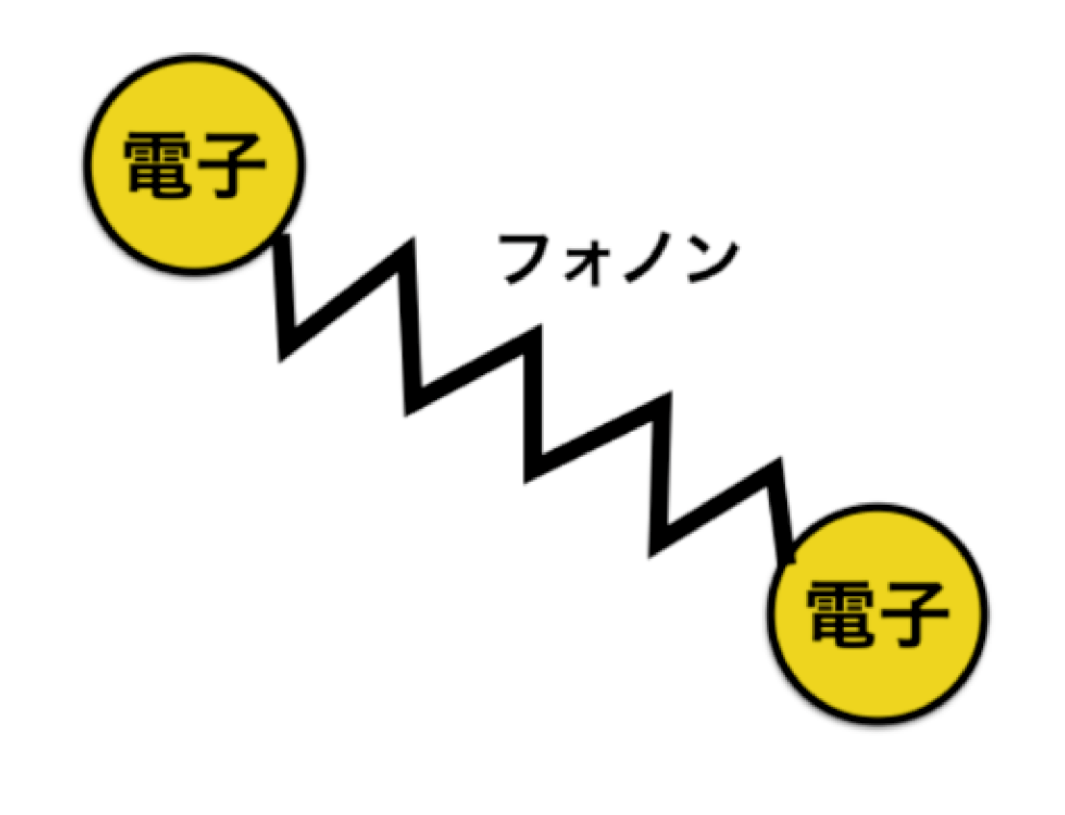
\includegraphics[width=9.0cm]{./Chapter/Chapter2/Picture/Cooperpair.eps}
    \caption{クーパー対概念図}
    \label{fig:CooperPair}
  \end{center}
\end{figure}

またボーズ$\cdot$アインシュタイン凝縮によりフェルミ準位近傍の電子は失われ、エネルギーギャップ$\Delta$が形成される。このエネルギーギャップ$\Delta$の2倍の$2 \Delta$が、クーパー対の結合エネルギーである。エネルギーギャップは超伝導体によって異なり、BCS理論から以下の関係が判明している。
\begin{eqnarray}
2 \Delta = 3.52 k_{B} T_{C}
\label{eq:E_Tc}
\end{eqnarray}
このことから、超伝導転移温度$\mathrm{T_C}$が小さいほど、エネルギーギャップ$\Delta$は小さくなることがわかる。
表\ref{tab:TcDelta}に異なる物質ごとのそれぞれの転移温度$T_C$とエネルギーギャップ$\Delta$を示した。

\begin{table}[htb]
	\begin{center}
		\caption{各物質ごとの転移温度$\mathrm{T_C}$とエネルギーギャップ$\Delta$}
		\begin{tabular}{| l || c | c | c | c |} \hline
			超伝導体 & Si & Nb & Al & Hf \\ \hline \hline
			転移温度$\mathrm{T_C}$[K] & - & 9.23 & 1.20 & 0.165 \\ \hline
			エネルギーギャップ$\Delta$[meV] & 1100 & 1.550 & 0.172 & 0.020 \\ \hline
		\end{tabular}
		\label{tab:TcDelta}
	\end{center}
\end{table}

	
\section{超電導トンネル接合素子光検出器(STJ)}

	\subsection{ジョセフソン効果}
	\begin{figure}[htbp]
  		\begin{center}
    			\includegraphics[width=9.0cm]{./Chapter/Chapter2/Picture/JosephsonJunction.eps}
    			\caption{ジョセフソン接合の概念図}
    			\label{fig:JosephsonJunction}
  		\end{center}
	\end{figure}
	図\ref{fig:JosephsonJunction}のように2つの超伝導体の間に非常に薄い絶縁体を持つSIS(Superconductor / Insulator / Superconductor)構造をもつ素子のことを超伝導トンネル接合素子(Superconducting Tunnel Junction : STJ)と呼ぶ。この素子の絶縁膜をトンネルするトンネル電流には以下の2種類のタイプが存在する。	
	\begin{itemize}
		\item クーパー対のトンネル効果によって流れる超伝導電流
		\item 励起された準粒子のトンネル効果による電流
	\end{itemize}	
	この1つ目の超伝導電流はジョセフソン電流と呼ばれている。このジョセフソン電流には、
	\begin{enumerate}
		\item 直流ジョセフソン電流
		\item 交流ジョセフソン電流
	\end{enumerate}
	の2種類存在する。以下、これらの電流について述べる。
		\subsubsection{直流ジョセフソン電流}
		前述にあるように、ボーズ粒子として振る舞うクーパー対はボーズ・アインシュタイン凝縮し、多数のクーパー対を同時に同一の波動関数、つまり巨視的波動関数で記述することができる。
		そして、図\ref{fig:JosephsonJunction}のような接合において左右の超伝導体でそれぞれ凝縮したクーパー対の系はそれぞれ巨視的波動関数で記述できる。
		ジョセフソン効果には、この位相の差$\delta \theta = \theta_{2} - \theta_{1}$が寄与し、電圧を印加していなくても、
		\begin{eqnarray}
			I = I_{0} \sin (\delta \theta)
			\label{eq:CriticalCurrent}
		\end{eqnarray}
		という超伝導電流が流れる。この$I_{0}$を臨界電流と呼ぶ。
		臨界電流以下なら接合の両端の位相差により、式(\ref{eq:CriticalCurrent})に従って電流が流れる。逆に$I_{0}$以下の電流を流すと式(\ref{eq:CriticalCurrent})に従った位相差が生じる。これを直流ジョセフソン電流という。
		\subsubsection{交流ジョセフソン電流}
		ジョセフソン接合における2つの超伝導体について、クーパー対がトンネルすることを考慮して波動方程式を立てると以下のようになる。
		\begin{eqnarray}
			i \hbar \frac{\partial \Psi_{1}}{\partial t} & = & \mu_{1} \Psi_{1} + K \Psi_{2} \\
			i \hbar \frac{\partial \Psi_{2}}{\partial t} & = & \mu_{2} \Psi_{2} + K \Psi_{1}
			\label{eq:ACJosephson}
		\end{eqnarray}
		
		これを平面解を仮定して解くと、以下のようになる。
		\begin{eqnarray}
			\hbar \frac{\partial n_1}{\partial t} = - \hbar \frac{\partial n_2}{\partial t} = 2 K {n_1}^{1/2} {n_2}^{1/2} \sin (\theta_2 - \theta_1) \\
			- \hbar \frac{\partial}{\partial t} (\theta_2 - \theta_1) = \mu_2 - \mu_1
			\label{eq:ACJosephson_phase}
		\end{eqnarray}
		$K$は2つの超伝導体の結合の強さを示し、$\mu_1$や$\mu_2$はそれぞれの超伝導体におけるクーパー対の化学ポテンシャル、$n_1$や$n_2$はそれぞれの超伝導体でのクーパー対の数密度である。ジョセフソン接合の両端に電位差$V$を与えたとき、接合の両端の位相差は式(\ref{eq:ACJosephson_phase})に従う。
		\begin{eqnarray}
		- \hbar \frac{\partial}{\partial t} \delta \theta = 2eV
		\label{eq:ACJosephson_phase_time}
		\end{eqnarray}
		式(\ref{eq:ACJosephson_phase_time})のように接合両端での位置エネルギー2eVに比例して位相差は時間発展する。このため接合には式(\ref{eq:ACJosephson})のような交流電流が流れる。
		\begin{eqnarray}
			I(t) = I_{0} \sin { \theta (0) - \frac{2eV}{\hbar} t }
			\label{eq:ACJosephson}
		\end{eqnarray}
		このとき周波数は式(\ref{eq:ACJosephson_fre})のようになる。
		\begin{eqnarray}
			2 \pi f = \frac{2eV}{h}
			\label{eq:ACJosephson_fre}
		\end{eqnarray}
		このように、直流電圧を印加することにより、交流電流が発生する現象のことを交流ジョセフソン効果といい、この交流電流のことを交流ジョセフソン電流と呼ぶ。そして、生じる交流の周波数は、$f = 483597.9 \mathrm{GHz/V}$で与えられ、この値をジョセフソン定数と呼ぶ。
	
	\subsection{STJ検出器の構造}
		\begin{figure}[htbp]
  			\begin{center}
    				%\includegraphics[width=9.0cm]{./Chapter/Chapter2/Picture/STJ_structure.eps}
    				\caption{超伝導トンネル接合素子光検出器(STJ検出器)\ 構造}
    				\label{fig:STJ_structure}
  			\end{center}
		\end{figure}
		STJの構造を図\ref{fig:STJ_structure}に示す。2枚の超伝導体は厚さ数100nm、大きさ数10〜数100$\mathrm{\mu m}$程度でその間を厚さ1nm程度の薄い絶縁体を挟んだSIS構造を持つ。素子の表面は$\mathrm{SiO_2}$の絶縁膜で覆われており、上部と下部の読み取りはコンタクトホールから配線が伸びて信号の読み出しを行う。
	
	\subsection{STJ検出器の動作原理}
		\begin{figure}[htbp]
  			\begin{center}
    				%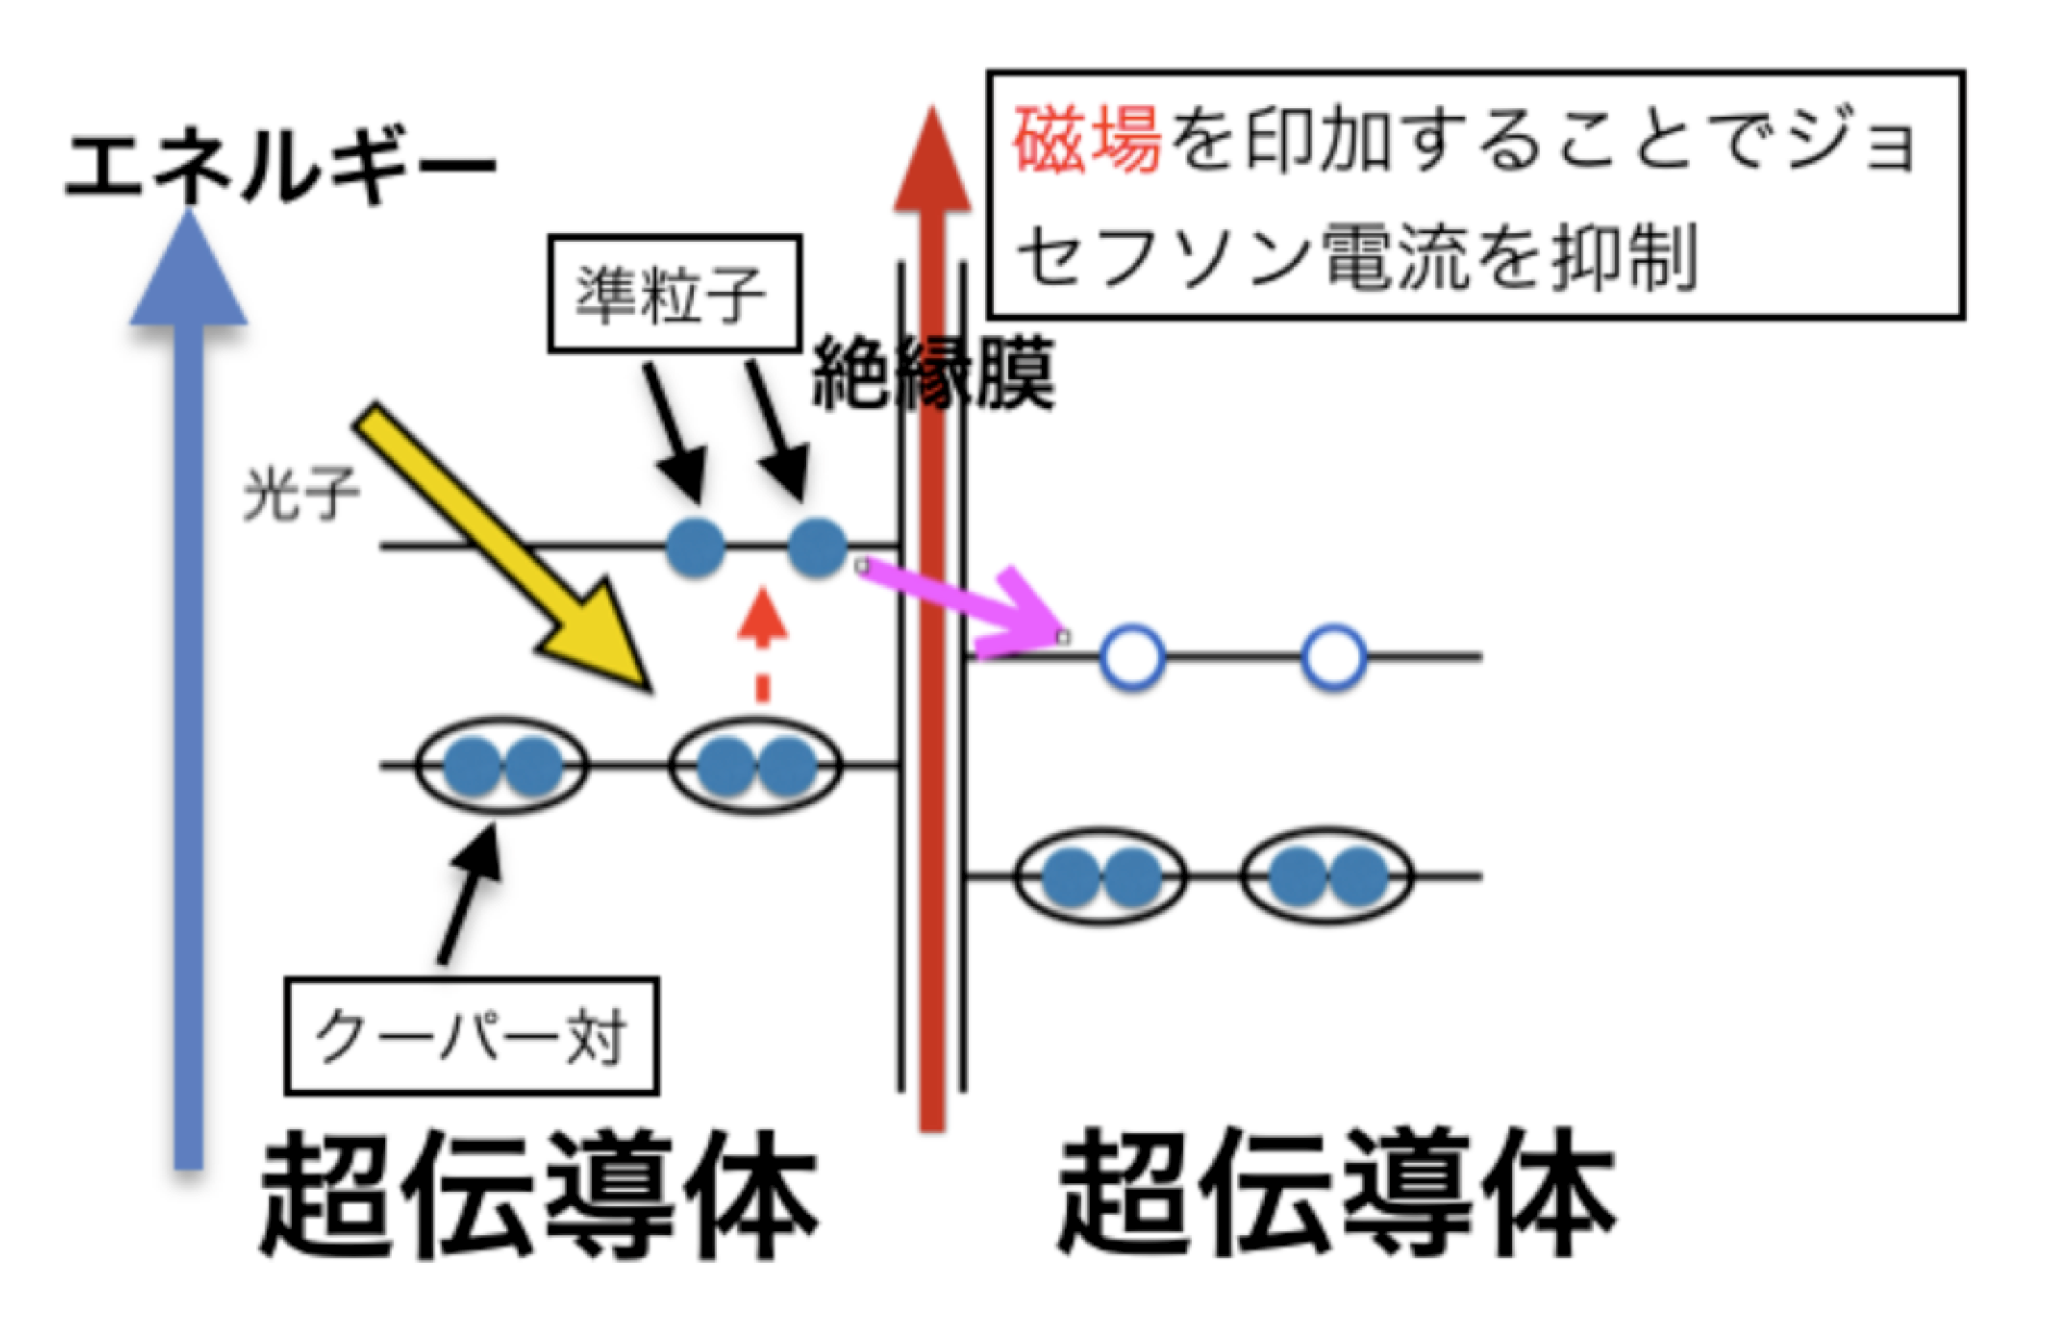
\includegraphics[width=12.0cm]{./Chapter/Chapter2/Picture/STJ_WorkingPrinciple.eps}
    				\caption{超伝導トンネル接合素子光検出器(STJ)動作原理の概念図}
    				\label{fig:STJ_WorkingPrinciple}
  			\end{center}
		\end{figure}
		STJ検出器の動作原理の概念図を図\ref{fig:STJ_WorkingPrinciple}に示す。粒子が検出器中に入射すると、超伝導体中のクーパー対が破壊され準粒子が生成される。生成された準粒子は超伝導体中を拡散し、絶縁膜に到達した準粒子はトンネル効果によって反対側の超伝導体へ通り抜ける。この準粒子のトンネル電流を信号として観測する。STJを動作する際には2つの超伝導体にバイアス電圧を印加し、2つの超伝導体の電位に勾配をつけることで絶縁膜をトンネルした準粒子の逆流を防ぐ。
		
		また、STJ検出器はSIS構造を持つので、信号とは別にジョセフソン電流も生じる。これは信号に対してバックグラウンドになるので抑制する必要がある。このジョセフソン電流は素子の絶縁膜に対して平行に磁場を印加した場合に抑制することができる。ジョセフソン電流$I_C$は磁場が存在すると、フラウンフォーファーと同型の依存性を示す。
		\begin{eqnarray}
			I_{C} = I_{C0} \left| \frac{\sin (\pi \phi / \phi_0)}{\pi \phi / \phi_0} \right|
		\end{eqnarray}
		$\phi$は印加磁場、$\phi_0$は定数である。磁場を印加することでジョセフソン電流が抑制されるので、STJ動作の際には十分な磁場を印加して、微弱な信号を観測する。
	
	\subsection{STJ検出器のエネルギー分解能}
		超伝導体状態ではフェルミオンである電子2つがフォノンを介してクーパー対を形成してボーズ粒子として振る舞う。STJを検出器として動作させる場合、入射粒子が超伝導体中のクーパー対を解離させ、2個の準粒子を生成し、それらの電子がトンネル効果で絶縁膜を通過することが必要になる。STJ信号を得るために必要な最低エネルギーは$2\Delta$である。したがって、$\Delta$が小さければ、それだけエネルギー分解能に優れた検出器ができる。STJのエネルギー分解能は式(\ref{eq:STJ_EnergyResolution})のように表される。
		\begin{eqnarray}
			\sigma_{FWHM} = \frac{\Delta N_q}{N_q} = 2.35 \sqrt{(1.7 \delta) FE}
			\label{eq:STJ_EnergyResolution}
		\end{eqnarray}
		ただし、
		\[
		\begin{cases}
			F : \mathrm{Fano\ Factor} \\
			E : \mathrm{入射粒子のエネルギー}
		\end{cases}
		\]
		である。Nb/Al-STJ検出器の場合、Fano\ Factorは0.1〜0.2程度である。式(\ref{eq:E_Tc})の関係式と照らし合わせて考察する。
		
		STJ検出器開発において、より高いエネルギー分解能が要求されるのに対し、エネルギー分解能を上げるためにエネルギーギャップが小さい超伝導体を用いようとすると、式(\ref{eq:E_Tc})から分かるように転移温度が低くなるので、より低温の測定系構築が要求されることになる。
		
	\subsection{STJのリーク電流}
		磁場を印加している場合、理想的なSTJ検出器ならば接合間に電流が流れることない。しかし、実際には以下で述べるような要因によるリーク電流が存在してしまい、これがSTJ信号のバックグラウンドとなる。
		\subsubsection{不完全な構造的な欠陥}
			酸化膜に開いた微小なピンホールや素子側面での2枚の超伝導体の接触などによるリーク電流をさす。図\ref{fig:STJ_leak_structure}にSTJ検出器の不完全な構造から生じるリーク電流の概念図を載せた。
			\begin{figure}[htbp]
  				\begin{center}
    					\includegraphics[width=12.0cm]{./Chapter/Chapter2/Picture/STJ_leak_structure.eps}
    					\caption{STJ検出器の不完全な構造起因の概念図}
    					\label{fig:STJ_leak_structure}
  				\end{center}
			\end{figure}	
		
		\subsubsection{熱励起によって生じる準粒子}
		構造的な欠陥をいくら改善しても、有限温度であれば必ず熱励起によって生じる準粒子は存在する。その準粒子がトンネル効果によって絶縁膜を流れるのならば、それはリーク電流となり得る。このリーク電流の温度依存性は理論的に計算されており、リーク電流$I_{\mathrm{leak}}$と温度$T$との関係は式(\ref{eq:STJ_leak_temp})のように書ける。\cite{13}
		\begin{eqnarray}
			I_{\mathrm{leak}} \propto T^{1/2} \exp \left(- \frac{\Delta}{k_{B}T} \right)
			\label{eq:STJ_leak_temp}
		\end{eqnarray}
		この式から、熱起因によるリーク電流は温度が下がるにつれて指数関数的に減少する。つまり、ここから言えることはSTJ検出器で十分なパフォーマンスを発揮するためには構造的な欠陥を極力抑えることに加えて、十分に冷却する必要もある。
		
		\subsubsection{その他}	
	
	\subsection{STJ検出器の電流電圧特性}
		\begin{figure}[htbp]
  			\begin{center}
    				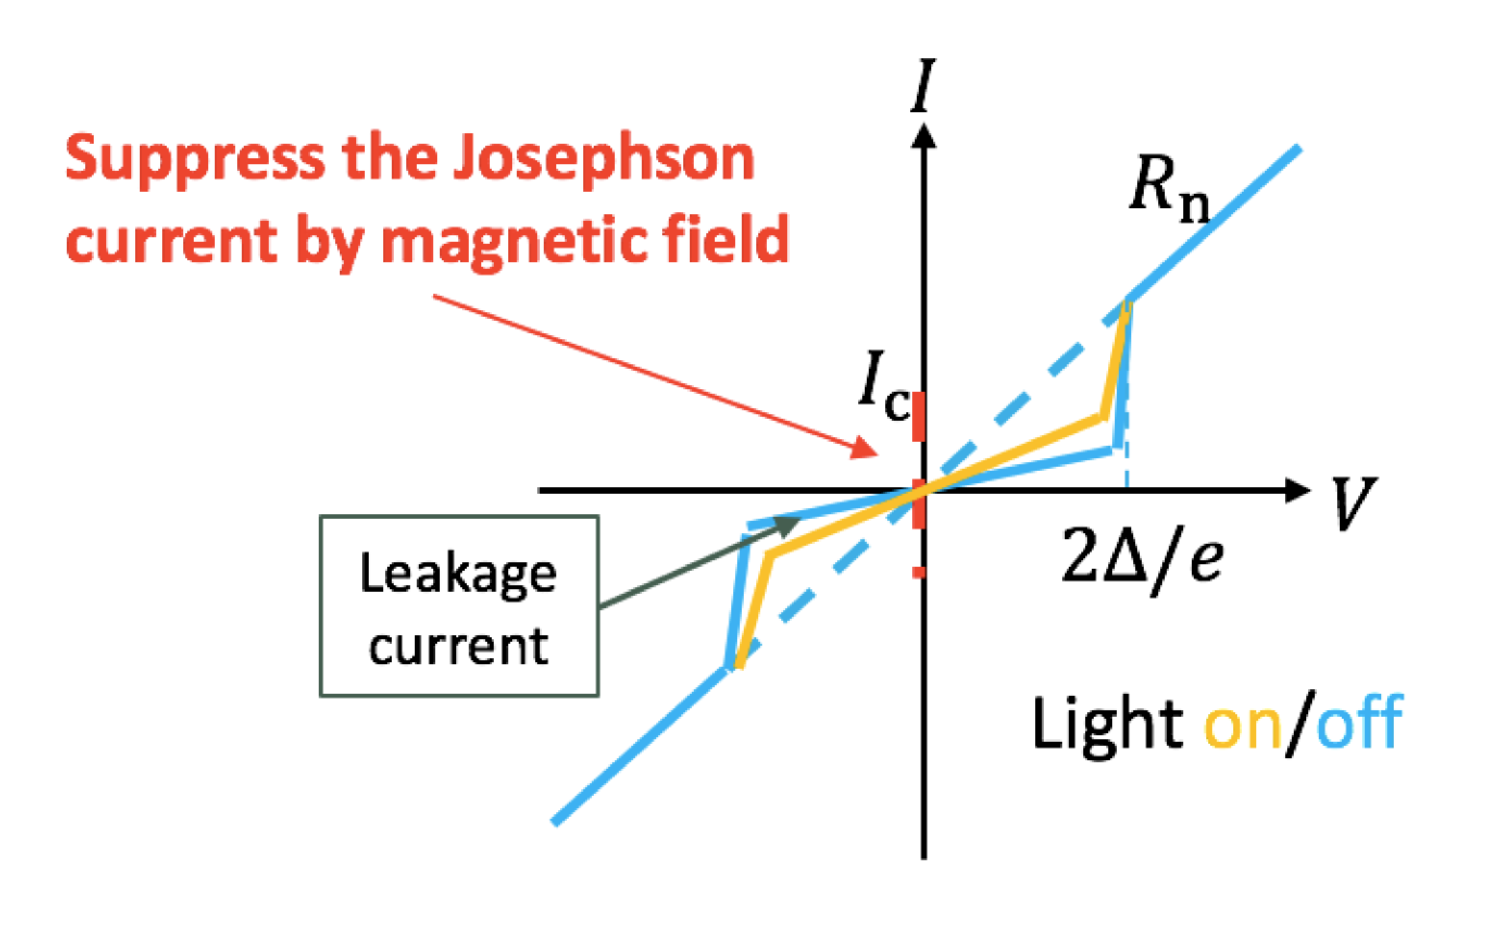
\includegraphics[width=12.0cm]{./Chapter/Chapter2/Picture/STJ_IV.eps}
    				\caption{一般的なSTJ検出器の電流電圧特性}
	  			\label{fig:STJ_IV}
  			\end{center}
		\end{figure}
		STJ検出器の電流電圧特性を図\ref{fig:STJ_IV}に示す。このSTJ検出器の電流電圧特性を測定し、素子の性能評価を行う。
		\begin{description}
			\item[$0 < |V| < 2 \Delta / e$の場合]\mbox{}\\
				クーパー対は準粒子として絶縁膜をトンネルすることができず、理想的には電流は流れない。しかし、前述したように不完全な構造や熱などに起因するリーク電流が存在するために、実際は電流はゼロにならず、有限の抵抗を持つ。この領域のことは「ダイナミックレジスタンス領域」と呼ばれ、そしてこの領域での抵抗値は$R_d$と表される。
			\item[$|V| > 2 \Delta /e$の場合]\mbox{}\\
				クーパー対はもう一方の超伝導体へトンネルすることができる。したがって、この領域での電流電圧特性は通常の抵抗のように振る舞う。この領域のことは「ノーマルレジスタンス領域」と呼ばれ、そしてこの領域での抵抗値は$R_n$と表される。
		\end{description}
		
		したがって、通常のSTJ検出器として動作させる場合は、印加電圧Vが「ダイナミックレジスタンス領域」に収まるように設定する。またSTJ検出器に光が入射した場合、クーパー対解離によって生じるトンネル電流が増加するので、図\ref{fig:STJ_IV}のように、青線から黄線に変化する。
	
\section{Nb/Al-STJ検出器}
	我々はニュートリノ崩壊光探索実験に用いるSTJ検出器として、超伝導体にハフニウムHfを用いた「Hf-STJ」と、超伝導体にニオブNbとアルミニウムAlを組み合わせた「Nb/Al-STJ」の研究開発を行っている。
	Hf-STJは、用いる超伝導体ハフニウムHfのエネルギーギャップ$\Delta$が0.020meVと非常に小さいのでエネルギー分解能に非常に優れている。我々は2012年に世界初のハフニウムHfを用いたHf-STJ検出器の作製に成功し、光に対する応答を確認した。このHf-STJは品質の良い素子作製プロセスを確立するために現在研究開発の最中である。また、これは将来の衛星実験の際に用いることを考えている。
	本節では、Hf-STJではなく、衛星実験の前実験であるロケット実験に用いるNb/Al-STJについて述べる。
	\subsection{Nb/Al-STJ検出器の構造}
		\begin{figure}[htbp]
  			\begin{center}
    				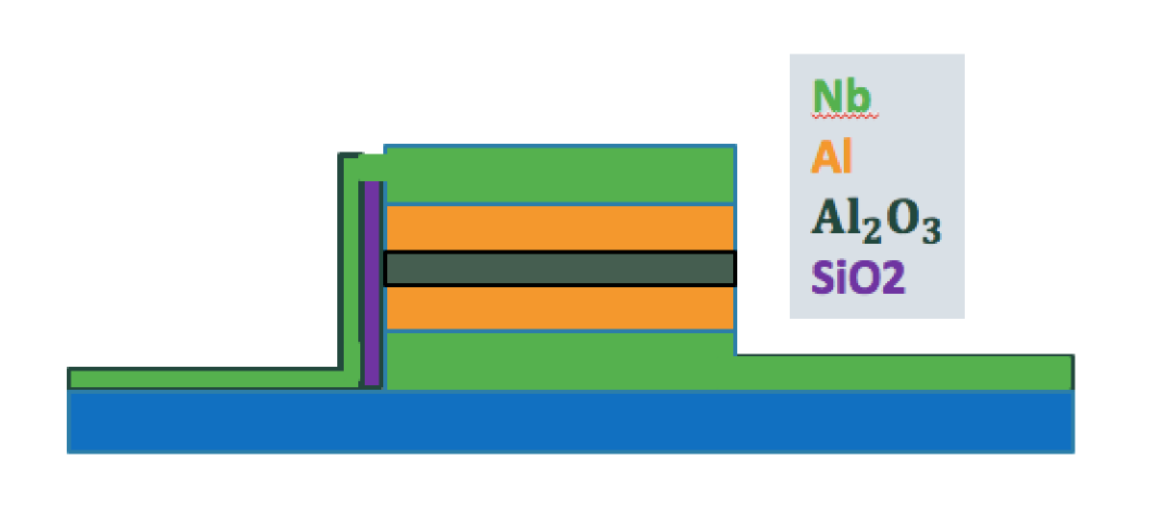
\includegraphics[width=12.0cm]{./Chapter/Chapter2/Picture/NbAlSTJ_structure.eps}
    				\caption{Nb/Al-STJ検出器の構造概念図}
	  			\label{fig:NbAlSTJ_structure}
  			\end{center}
		\end{figure}
		前述したように、Nb/Al-STJ検出器はニュートリノ崩壊光探索ロケット実験に用いる予定で、現在研究開発中である。用いる超伝導体に、ニオブNbとアルミニウムAlの2種類の超伝導体を組み合わせており、絶縁膜に酸化アルミニウム$\mathrm{Al_{2}O_3}$を用いている。Nb/Al-STJ検出器の構造を図\ref{fig:NbAlSTJ_structure}に示す。
		ニオブNb層と絶縁膜の間に、ニオブNbのエネルギーギャップ$\Delta_{\mathrm{Nb}}$に比べて更にエネルギーギャップが小さいアルミニウムAl層を挟むことによって、STJ検出器として動作させる際に有利に働く以下の特徴が現れる。
		\begin{description}
			\item[より高品質な絶縁膜の形成]\mbox{}\\
				Nb酸化膜を絶縁膜としたSTJ検出器は熱サイクルに弱く、繰り返し冷却して使用できない。一方、Al酸化膜は熱サイクルに強い。\\
				使い勝手のよいSTJ検出器を作製するために、Al酸化膜をNb系STJ検出器に用いる場合、必然的にニオブNb層とAl酸化膜の間にAl層を形成することになる。
			\item[近接効果による転移温度$T_C$とエネルギーギャップ$\Delta$の調節]\mbox{}\\
				ニオブの転移温度$T_{C\mathrm{Nb}}$が9.2Kであるのに対し、アルミニウムの転移温度$T_{C\mathrm{Al}}$は1.1Kと低い。
				2つの超伝導体を接合した場合、一方の超伝導体のクーパー対の波動関数がもう一方の超伝導体内に染み出し、転移温度が変化する。
				この効果を「近接効果」という。変化の度合いは2つの超伝導体の厚みの比率に応じて変化する。
				式(\ref{eq:E_Tc})と照らし合わせて考えると、Al層の厚さを調節することによって、転移温度と、同時にエネルギーギャップ$\Delta$を調節することができる。
				したがって、Al層を挟むことによって、Nb単体で作製されたSTJ検出器に比べてエネルギーギャップ$\Delta$は下がる。
				結果エネルギー分解能を向上させることが可能である。
			\item[バックトンネリングによるトンネル準粒子数の増加]\mbox{}\\
				\begin{figure}[htbp]
  					\begin{center}
    						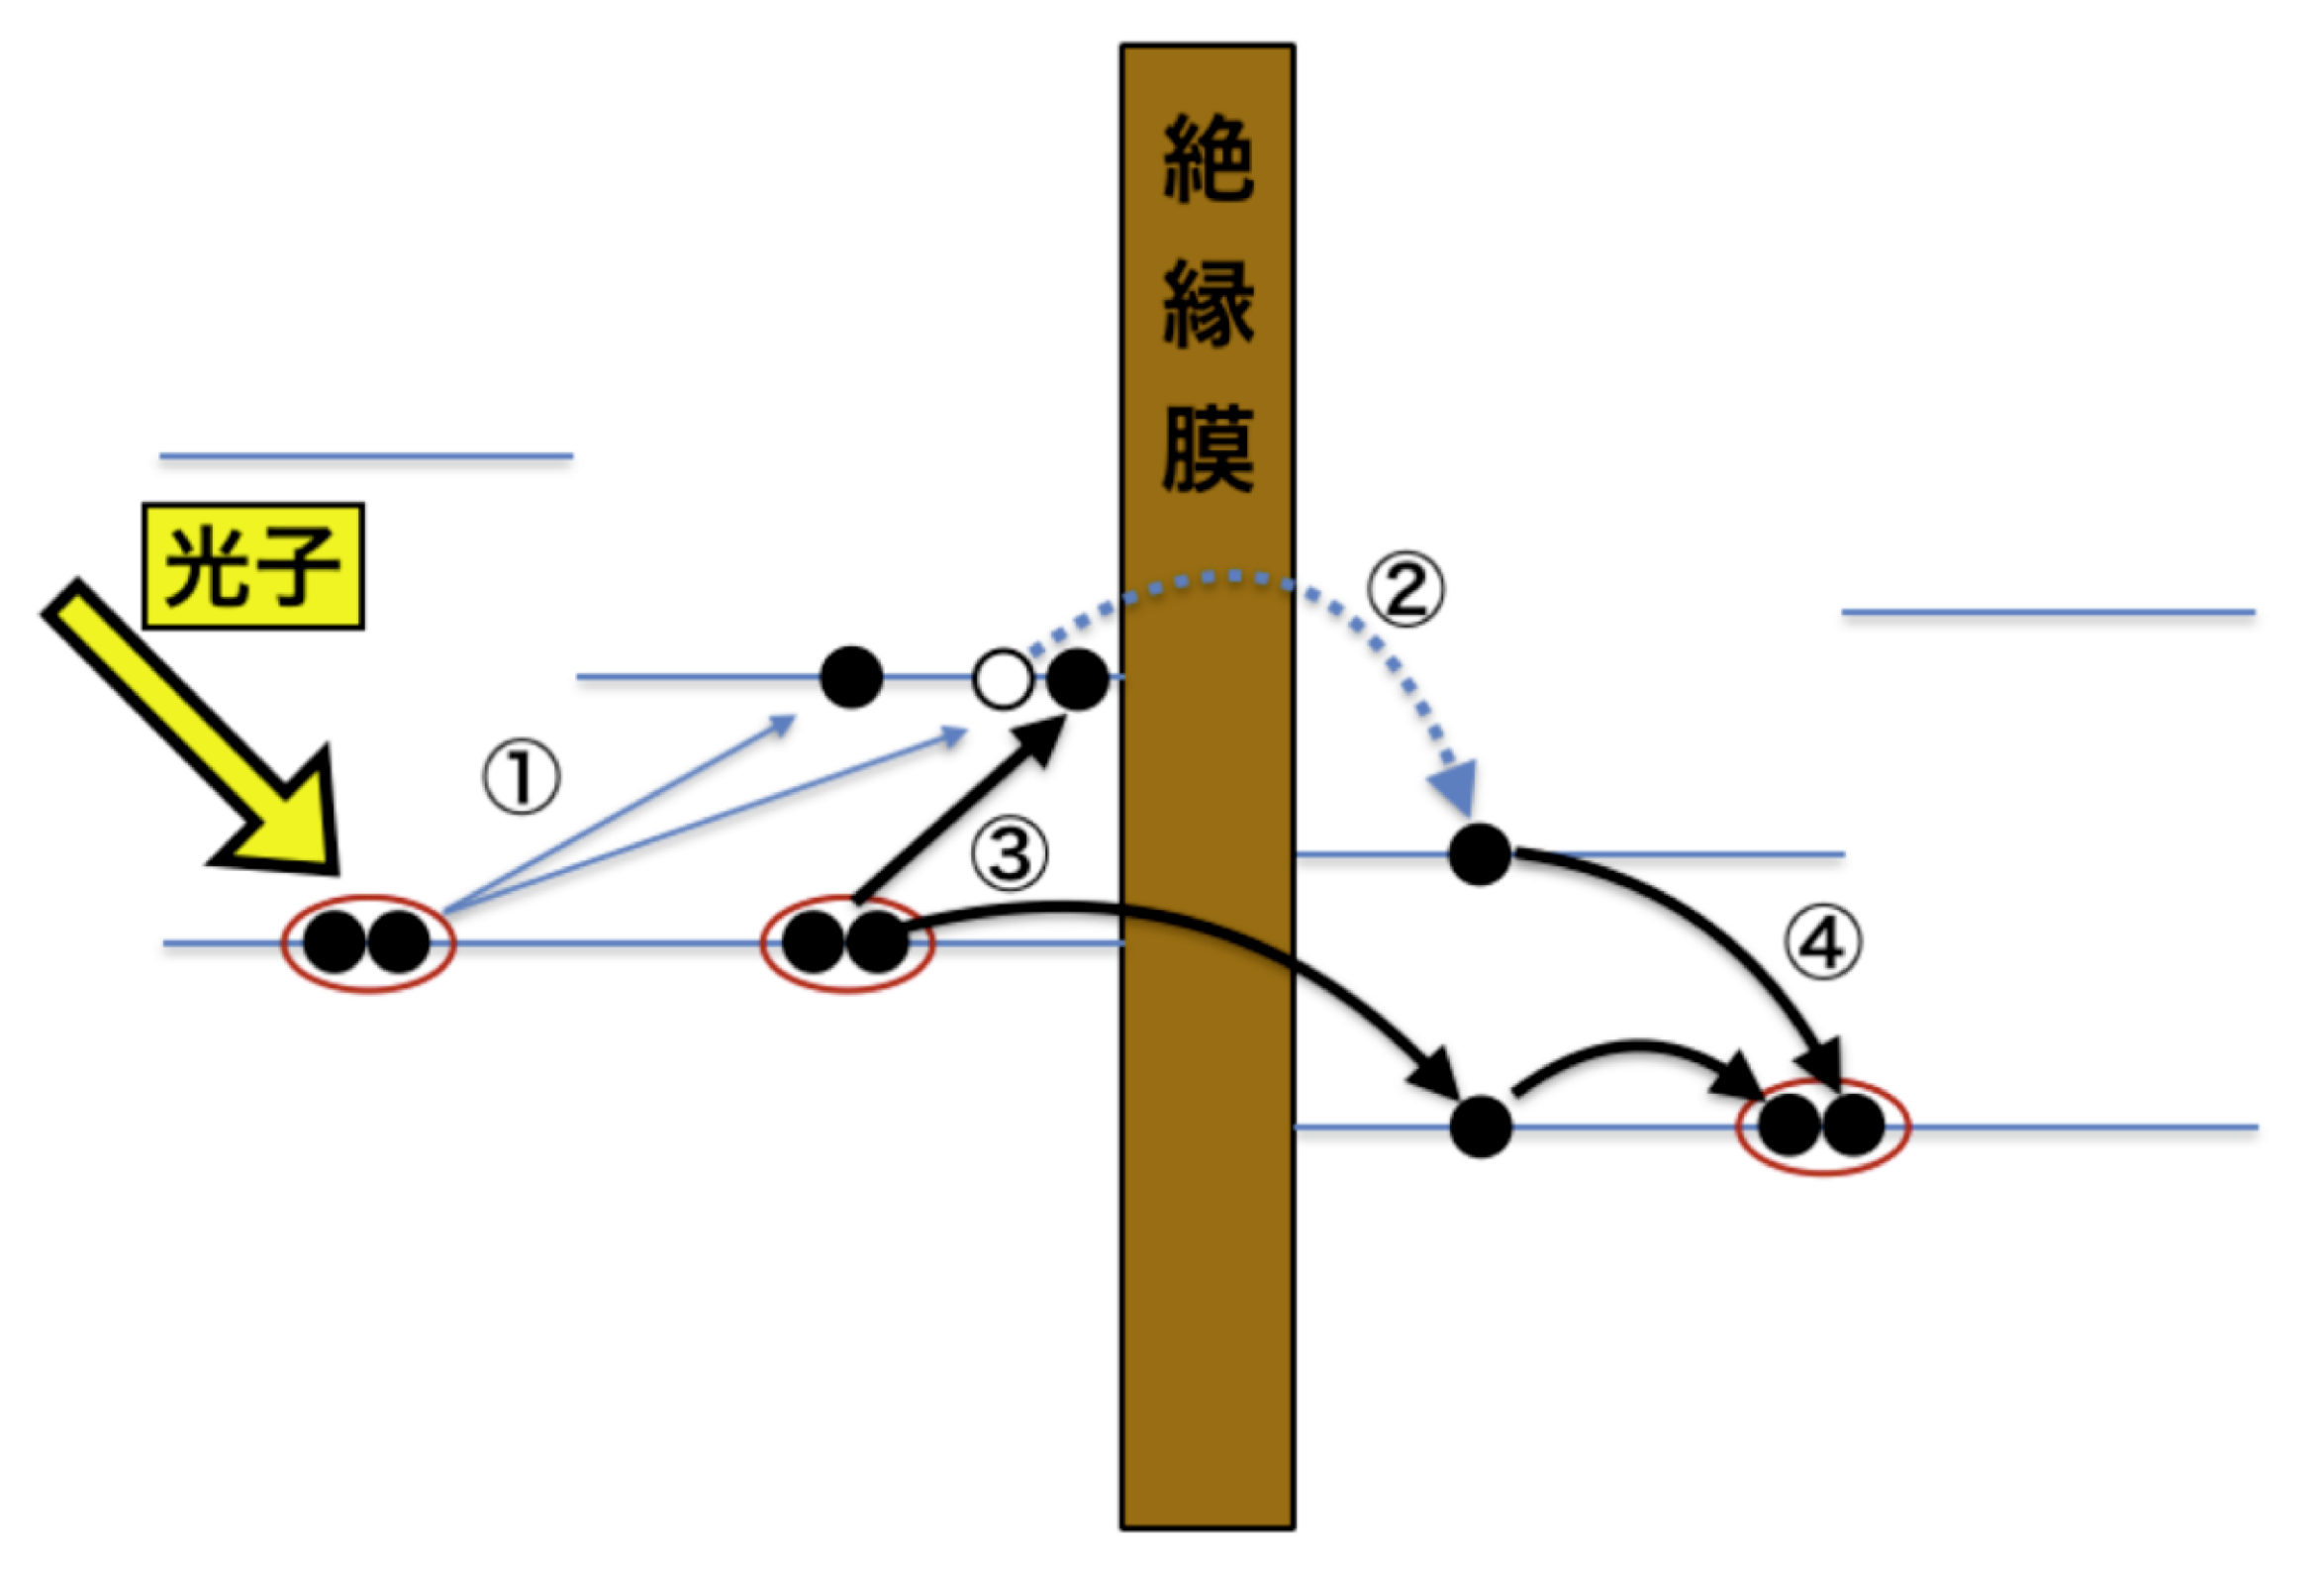
\includegraphics[width=12.0cm]{./Chapter/Chapter2/Picture/NbAlSTJ_backtunnel.eps}
    						\caption{バックトンネリング効果の概念図}
	  					\label{fig:NbAlSTJ_backtunnel}
  					\end{center}
				\end{figure}
				Nb/Al-STJ検出器のように、超伝導体と絶縁膜の間によりエネルギーギャップが小さい超伝導体を挟むことでトンネルする準粒子数が増加する、バックトンネリング効果が現れる。図\ref{fig:NbAlSTJ_backtunnel}にバックトンネリング効果の概念図を載せる。
				
				バックトンネリング効果の流れは以下のようになる。
				\begin{enumerate}
					\item STJ検出器の上部伝導体に入射した粒子がクーパー対を壊し、2つの準粒子を発生させる。
					\item 2つの準粒子のうち、1つは上部超伝導体のAl層の常伝導体にトラップされて、もう1つは絶縁膜をトンネルして下部聴伝導体のAl層の常伝導体にトラップされる。
					\item 下部超伝導体にクーパー対を作ろうと、上部伝導体の別のクーパー対が壊されて新たに2つの準粒子が生成される。
					\item 先に絶縁膜をトンネルした粒子どうしが再結合してクーパー対をなす。
					\item 残された準粒子は上部超伝導体のAl層常伝導体でトラップされる
				\end{enumerate}
				この一連の流れを繰り返すことでトンネル準粒子数が増加、つまりトンネル電流が増加する。
				バックトンネリング効果を踏まえ、STJ検出器にエネルギーEを持つ粒子が入射したときの準粒子生成個数$N$は、
				\begin{eqnarray}
					N = G_{\mathrm{Al}} \frac{E}{1.7 \Delta}
				\end{eqnarray}
				となる。この$G_{\mathrm{Al}}$をトラッピングゲインと呼び、バックトンネリング効果によるトンネル準粒子数の増加率を表す。トラッピングゲイン$G_{\mathrm{Al}}$は約10倍程度とされている。
		\end{description}

	\subsection{Nb/Al-STJ検出器の研究開発の現状}
		本研究グループは2014年度から、産業技術総合研究所(AIST)との共同研究を開始した。
		そして、Nb/Al-STJ検出器素子作製は産業技術総合研究所のCRAVITY(Clean Room for Analog-digital superconductiVITY)で行なわれている。
		ここでは安定して高品質の超伝導素子を作製することができる。
		
		図\ref{fig:NbAlSTJ_leaktemp}にCRAVITYで作製されたNb/Al-STJ検出器のリーク電流の温度依存性を示す。
		素子のサイズは$50 \times 50 \mathrm{{\mu m}^2}$である。
		この図からわかるように、0.4K程度以下でリーク電流が飽和することがわかる。この飽和したリーク電流は熱起因ではないリーク電流であり、より高品質のSTJ検出器素子作製や測定系の改善を行うことで下げることができる。
		25meVの一光子をリーク電流の揺らぎに対して$3 \sigma$以上で検出するためには、STJ検出器の信号幅を$1 \mathrm{\mu s}$と仮定すると、STJ検出器のリーク電流要求値は100pA以下である必要がある。
		表\ref{tab:NbAlSTJ_leaksize}に、我々が測定したNb/Al-STJ検出器のサイズごとのリーク電流値を示す。この表からCRAVITY製のNb/Al-STJ検出器はCOBAND実験のリーク電流の要求値を満たしていることがわかる。
		
		しかし、現在もなおNb/Al-STJ検出器を用いて遠赤外光一光子検出の成功には至っていない。その理由として、STJ検出器からの信号を冷凍機外部へと長い配線を経て読み出す際に、測定系由来の雑音がSTJ検出器信号に大きく効いてきてしまうからだ。この問題の解決策として、STJ検出器が動作する極低温環境下においても動作可能な前置増幅器を冷凍機内に設置し、STJ検出器信号が雑音に埋もれてしまう前に増幅する方法がある。\\
		我々は現在、この極低温前置増幅器の研究開発を行なっており、次章はこれについて詳しく述べる。
		%=====Nb/Al-STJのリーク電流温度依存性のplotを載せる=====%
		\begin{figure}[htbp]
  			\begin{center}
  				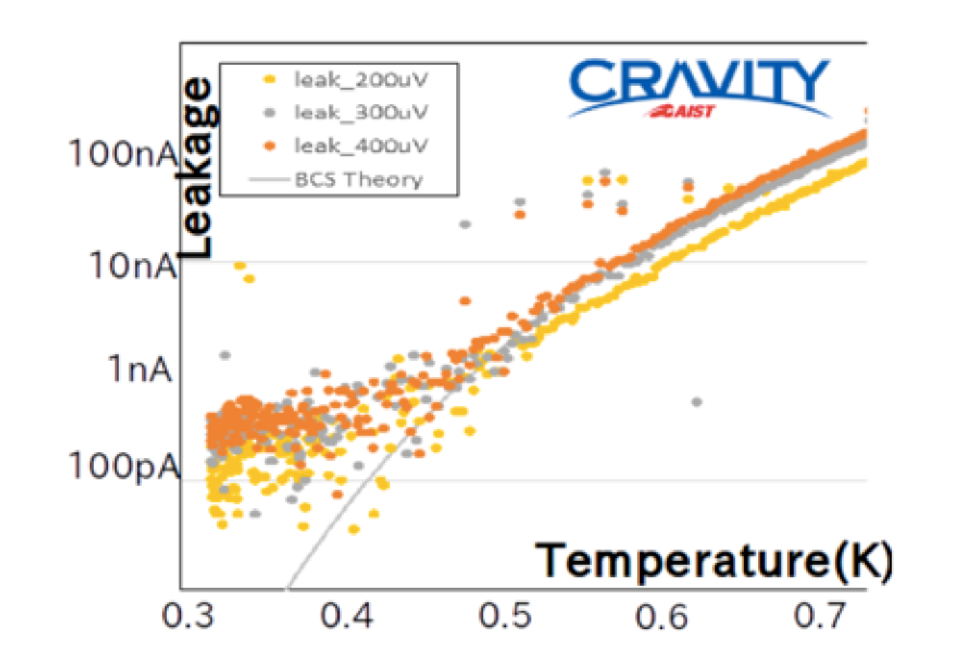
\includegraphics[width=8.0cm]{./Chapter/Chapter2/Picture/NbAlSTJ_leaktemp.eps}
    				\caption{CRAVITY製Nb/Al-STJ検出器のリーク電流温度依存性}
	  			\label{fig:NbAlSTJ_leaktemp}
 			\end{center}
		\end{figure}
		%=====現在のリーク電流の状況を表にして載せる=====%
		\begin{table}[htb]
			\begin{center}
				\caption{CRAVITY製Nb/Al-STJ検出器のサイズごとのリーク電流値}
				\begin{tabular}{| l || c | c | c |} \hline
					Nb/Al-STJのサイズ & ${100 \mathrm{\mu m}}^2$ & ${50 \mathrm{\mu m}}^2$ & ${20 \mathrm{\mu m}}^2$ \\ \hline
					リーク電流$I_{\mathrm{leak}}$@0.4mV & 2 nA & 300 pA & 100 pA \\ \hline
				\end{tabular}
				\label{tab:NbAlSTJ_leaksize}
			\end{center}
		\end{table}




%%%%%%%%%%%%%%%%%%%%%%%%%%%%%%%%%%%%%%%%%%%%%%%%%%%%%%%%%%%%%%%
\chapter{超伝導トンネル接合素子光検出器(STJ)}
前章で述べたように、ニュートリノ崩壊から放出される光子のエネルギーは25meVであると予想されている。したがって用いる検出器への要求は、
\begin{enumerate}
\item 25meVのエネルギー領域で感度を持つこと
\item エネルギースペクトルからニュートリノ崩壊光として評価するためにはエネルギー分解能$2 \%$を達成すること
\end{enumerate}
が必要である。

一方、検出器のエネルギー分解能はその物質のエネルギーギャップによって決まるが、通常の半導体検出器では前述した要求を満たさず、検出器開発は不可能であると考えられる。
したがって、我々は上記の要求を達成するために、ニュートリノ崩壊光探索実験において、超伝導トンネル接合素子光検出器(STJ : Superconducting Tunnel Junction、以下「STJ」と表記する)を用いる。STJとは、非常に薄い絶縁膜を2つの超伝導体で挟んだ構造をしており、超伝導体の転移温度以下で動作可能な検出器である。半導体に比べて非常にエネルギーギャップが小さいので、目標のエネルギー分解能を達成することができると考え、研究開発を進めている。
本章では、STJについて説明し、我々が研究開発しているNb/Al-STJ検出器開発について述べる。
\section{超伝導の基礎}
超伝導体の示す基本的な実験事実として、「完全電気伝導性」と「完全反磁性」の2つを述べる。
	\begin{description}
	\item[完全電気伝導性]\mbox{}\\
		1911年、オランダのH.Kamerlingh Onnesは水銀を液体ヘリウムで冷却して行った時、温度4.2Kで突然電気抵抗が下がり、4.19Kで$10^{-5} \Omega$以下になる現象を報告した。その後、水銀以外にも特定の金属や合金に対し、温度を下げていくと突然急激に電気抵抗が下がりほぼ0になる性質を持つことが発見された。このように電気抵抗が急激に落ちて0になる超伝導体特有の性質を「完全電気伝導性」と呼び、そしてこの時の温度のことを臨界温度(critical temperature)、または転移温度(transition temperature)といい、$\mathrm{T_C}$と表す。
	\item[完全反磁性]\mbox{}\\
		1933年にF.Walther Meissnerによって超伝導体に完全反磁性を示すことが発見された。この効果をMeissner効果と呼び、超伝導体内部では磁場が排除される。
	\end{description}
	
超伝導現象の基礎になる理論は1957年にJ.Bardeen、L. N. Cooper、J. M. Schriefferによって発見され、この理論のことを頭文字をとって、「BCS理論」という。この理論では、臨界温度$\mathrm{T_C}$以下の温度において電子$\cdot$格子相互作用を介して電子対のスピンが互いに逆向き、対の角運動量の合計がゼロの状態が形成され、これらの電子同士に引力が働くと考えられている。BCS理論では図\ref{fig:CooperPair}のように電子$\cdot$格子相互作用を介して電子同士がフォノンを仮想的に交換することによって引力が働くと考える。その引力によって結合している電子対のことをクーパー対(cooper pair)と呼ぶ。電子$\cdot$電子対のクーパー対は運動量、スピンがゼロのボーズ粒子として振る舞い、ボーズ$\cdot$アインシュタイン凝縮を起こし1つの量子状態へ落ち込む。多数のクーパー対が同じ状態に落ち込むということは、つまり多数のクーパー対を同時に同一の波動関数で記述できる。この波動関数を巨視的波動関数という。

\begin{eqnarray}
\Phi (\bm{r},t) = |\Phi (\bm{r},t)| \exp (i \theta (\bm{r},t))
\end{eqnarray}

\begin{figure}[htbp]
  \begin{center}
    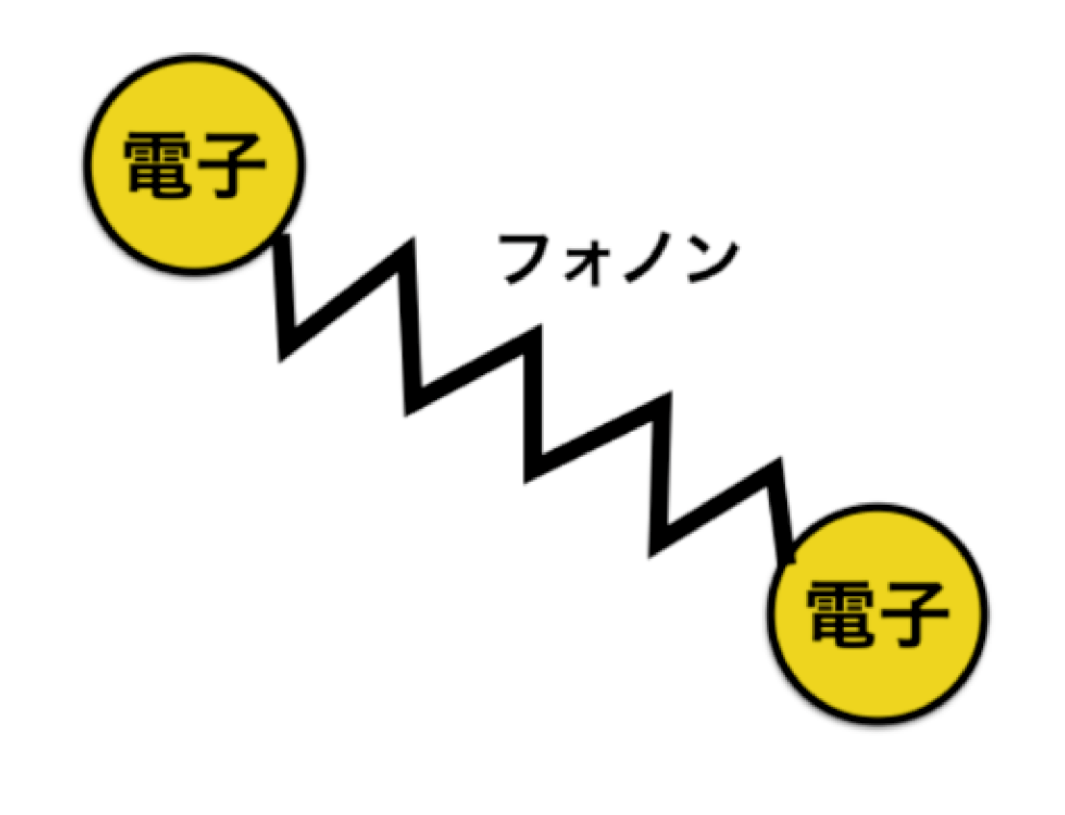
\includegraphics[width=9.0cm]{./Chapter/Chapter2/Picture/Cooperpair.eps}
    \caption{クーパー対概念図}
    \label{fig:CooperPair}
  \end{center}
\end{figure}

またボーズ$\cdot$アインシュタイン凝縮によりフェルミ準位近傍の電子は失われ、エネルギーギャップ$\Delta$が形成される。このエネルギーギャップ$\Delta$の2倍の$2 \Delta$が、クーパー対の結合エネルギーである。エネルギーギャップは超伝導体によって異なり、BCS理論から以下の関係が判明している。
\begin{eqnarray}
2 \Delta = 3.52 k_{B} T_{C}
\label{eq:E_Tc}
\end{eqnarray}
このことから、超伝導転移温度$\mathrm{T_C}$が小さいほど、エネルギーギャップ$\Delta$は小さくなることがわかる。
表\ref{tab:TcDelta}に異なる物質ごとのそれぞれの転移温度$T_C$とエネルギーギャップ$\Delta$を示した。

\begin{table}[htb]
	\begin{center}
		\caption{各物質ごとの転移温度$\mathrm{T_C}$とエネルギーギャップ$\Delta$}
		\begin{tabular}{| l || c | c | c | c |} \hline
			超伝導体 & Si & Nb & Al & Hf \\ \hline \hline
			転移温度$\mathrm{T_C}$[K] & - & 9.23 & 1.20 & 0.165 \\ \hline
			エネルギーギャップ$\Delta$[meV] & 1100 & 1.550 & 0.172 & 0.020 \\ \hline
		\end{tabular}
		\label{tab:TcDelta}
	\end{center}
\end{table}

	
\section{超電導トンネル接合素子光検出器(STJ)}

	\subsection{ジョセフソン効果}
	\begin{figure}[htbp]
  		\begin{center}
    			\includegraphics[width=9.0cm]{./Chapter/Chapter2/Picture/JosephsonJunction.eps}
    			\caption{ジョセフソン接合の概念図}
    			\label{fig:JosephsonJunction}
  		\end{center}
	\end{figure}
	図\ref{fig:JosephsonJunction}のように2つの超伝導体の間に非常に薄い絶縁体を持つSIS(Superconductor / Insulator / Superconductor)構造をもつ素子のことを超伝導トンネル接合素子(Superconducting Tunnel Junction : STJ)と呼ぶ。この素子の絶縁膜をトンネルするトンネル電流には以下の2種類のタイプが存在する。	
	\begin{itemize}
		\item クーパー対のトンネル効果によって流れる超伝導電流
		\item 励起された準粒子のトンネル効果による電流
	\end{itemize}	
	この1つ目の超伝導電流はジョセフソン電流と呼ばれている。このジョセフソン電流には、
	\begin{enumerate}
		\item 直流ジョセフソン電流
		\item 交流ジョセフソン電流
	\end{enumerate}
	の2種類存在する。以下、これらの電流について述べる。
		\subsubsection{直流ジョセフソン電流}
		前述にあるように、ボーズ粒子として振る舞うクーパー対はボーズ・アインシュタイン凝縮し、多数のクーパー対を同時に同一の波動関数、つまり巨視的波動関数で記述することができる。
		そして、図\ref{fig:JosephsonJunction}のような接合において左右の超伝導体でそれぞれ凝縮したクーパー対の系はそれぞれ巨視的波動関数で記述できる。
		ジョセフソン効果には、この位相の差$\delta \theta = \theta_{2} - \theta_{1}$が寄与し、電圧を印加していなくても、
		\begin{eqnarray}
			I = I_{0} \sin (\delta \theta)
			\label{eq:CriticalCurrent}
		\end{eqnarray}
		という超伝導電流が流れる。この$I_{0}$を臨界電流と呼ぶ。
		臨界電流以下なら接合の両端の位相差により、式(\ref{eq:CriticalCurrent})に従って電流が流れる。逆に$I_{0}$以下の電流を流すと式(\ref{eq:CriticalCurrent})に従った位相差が生じる。これを直流ジョセフソン電流という。
		\subsubsection{交流ジョセフソン電流}
		ジョセフソン接合における2つの超伝導体について、クーパー対がトンネルすることを考慮して波動方程式を立てると以下のようになる。
		\begin{eqnarray}
			i \hbar \frac{\partial \Psi_{1}}{\partial t} & = & \mu_{1} \Psi_{1} + K \Psi_{2} \\
			i \hbar \frac{\partial \Psi_{2}}{\partial t} & = & \mu_{2} \Psi_{2} + K \Psi_{1}
			\label{eq:ACJosephson}
		\end{eqnarray}
		
		これを平面解を仮定して解くと、以下のようになる。
		\begin{eqnarray}
			\hbar \frac{\partial n_1}{\partial t} = - \hbar \frac{\partial n_2}{\partial t} = 2 K {n_1}^{1/2} {n_2}^{1/2} \sin (\theta_2 - \theta_1) \\
			- \hbar \frac{\partial}{\partial t} (\theta_2 - \theta_1) = \mu_2 - \mu_1
			\label{eq:ACJosephson_phase}
		\end{eqnarray}
		$K$は2つの超伝導体の結合の強さを示し、$\mu_1$や$\mu_2$はそれぞれの超伝導体におけるクーパー対の化学ポテンシャル、$n_1$や$n_2$はそれぞれの超伝導体でのクーパー対の数密度である。ジョセフソン接合の両端に電位差$V$を与えたとき、接合の両端の位相差は式(\ref{eq:ACJosephson_phase})に従う。
		\begin{eqnarray}
		- \hbar \frac{\partial}{\partial t} \delta \theta = 2eV
		\label{eq:ACJosephson_phase_time}
		\end{eqnarray}
		式(\ref{eq:ACJosephson_phase_time})のように接合両端での位置エネルギー2eVに比例して位相差は時間発展する。このため接合には式(\ref{eq:ACJosephson})のような交流電流が流れる。
		\begin{eqnarray}
			I(t) = I_{0} \sin { \theta (0) - \frac{2eV}{\hbar} t }
			\label{eq:ACJosephson}
		\end{eqnarray}
		このとき周波数は式(\ref{eq:ACJosephson_fre})のようになる。
		\begin{eqnarray}
			2 \pi f = \frac{2eV}{h}
			\label{eq:ACJosephson_fre}
		\end{eqnarray}
		このように、直流電圧を印加することにより、交流電流が発生する現象のことを交流ジョセフソン効果といい、この交流電流のことを交流ジョセフソン電流と呼ぶ。そして、生じる交流の周波数は、$f = 483597.9 \mathrm{GHz/V}$で与えられ、この値をジョセフソン定数と呼ぶ。
	
	\subsection{STJ検出器の構造}
		\begin{figure}[htbp]
  			\begin{center}
    				\includegraphics[width=9.0cm]{./Chapter/Chapter2/Picture/STJ_structure.eps}
    				\caption{超伝導トンネル接合素子光検出器(STJ検出器)\ 構造}
    				\label{fig:STJ_structure}
  			\end{center}
		\end{figure}
		STJの構造を図\ref{fig:STJ_structure}に示す。2枚の超伝導体は厚さ数100nm、大きさ数10〜数100$\mathrm{\mu m}$程度でその間を厚さ1nm程度の薄い絶縁体を挟んだSIS構造を持つ。素子の表面は$\mathrm{SiO_2}$の絶縁膜で覆われており、上部と下部の読み取りはコンタクトホールから配線が伸びて信号の読み出しを行う。
	
	\subsection{STJ検出器の動作原理}
		\begin{figure}[htbp]
  			\begin{center}
    				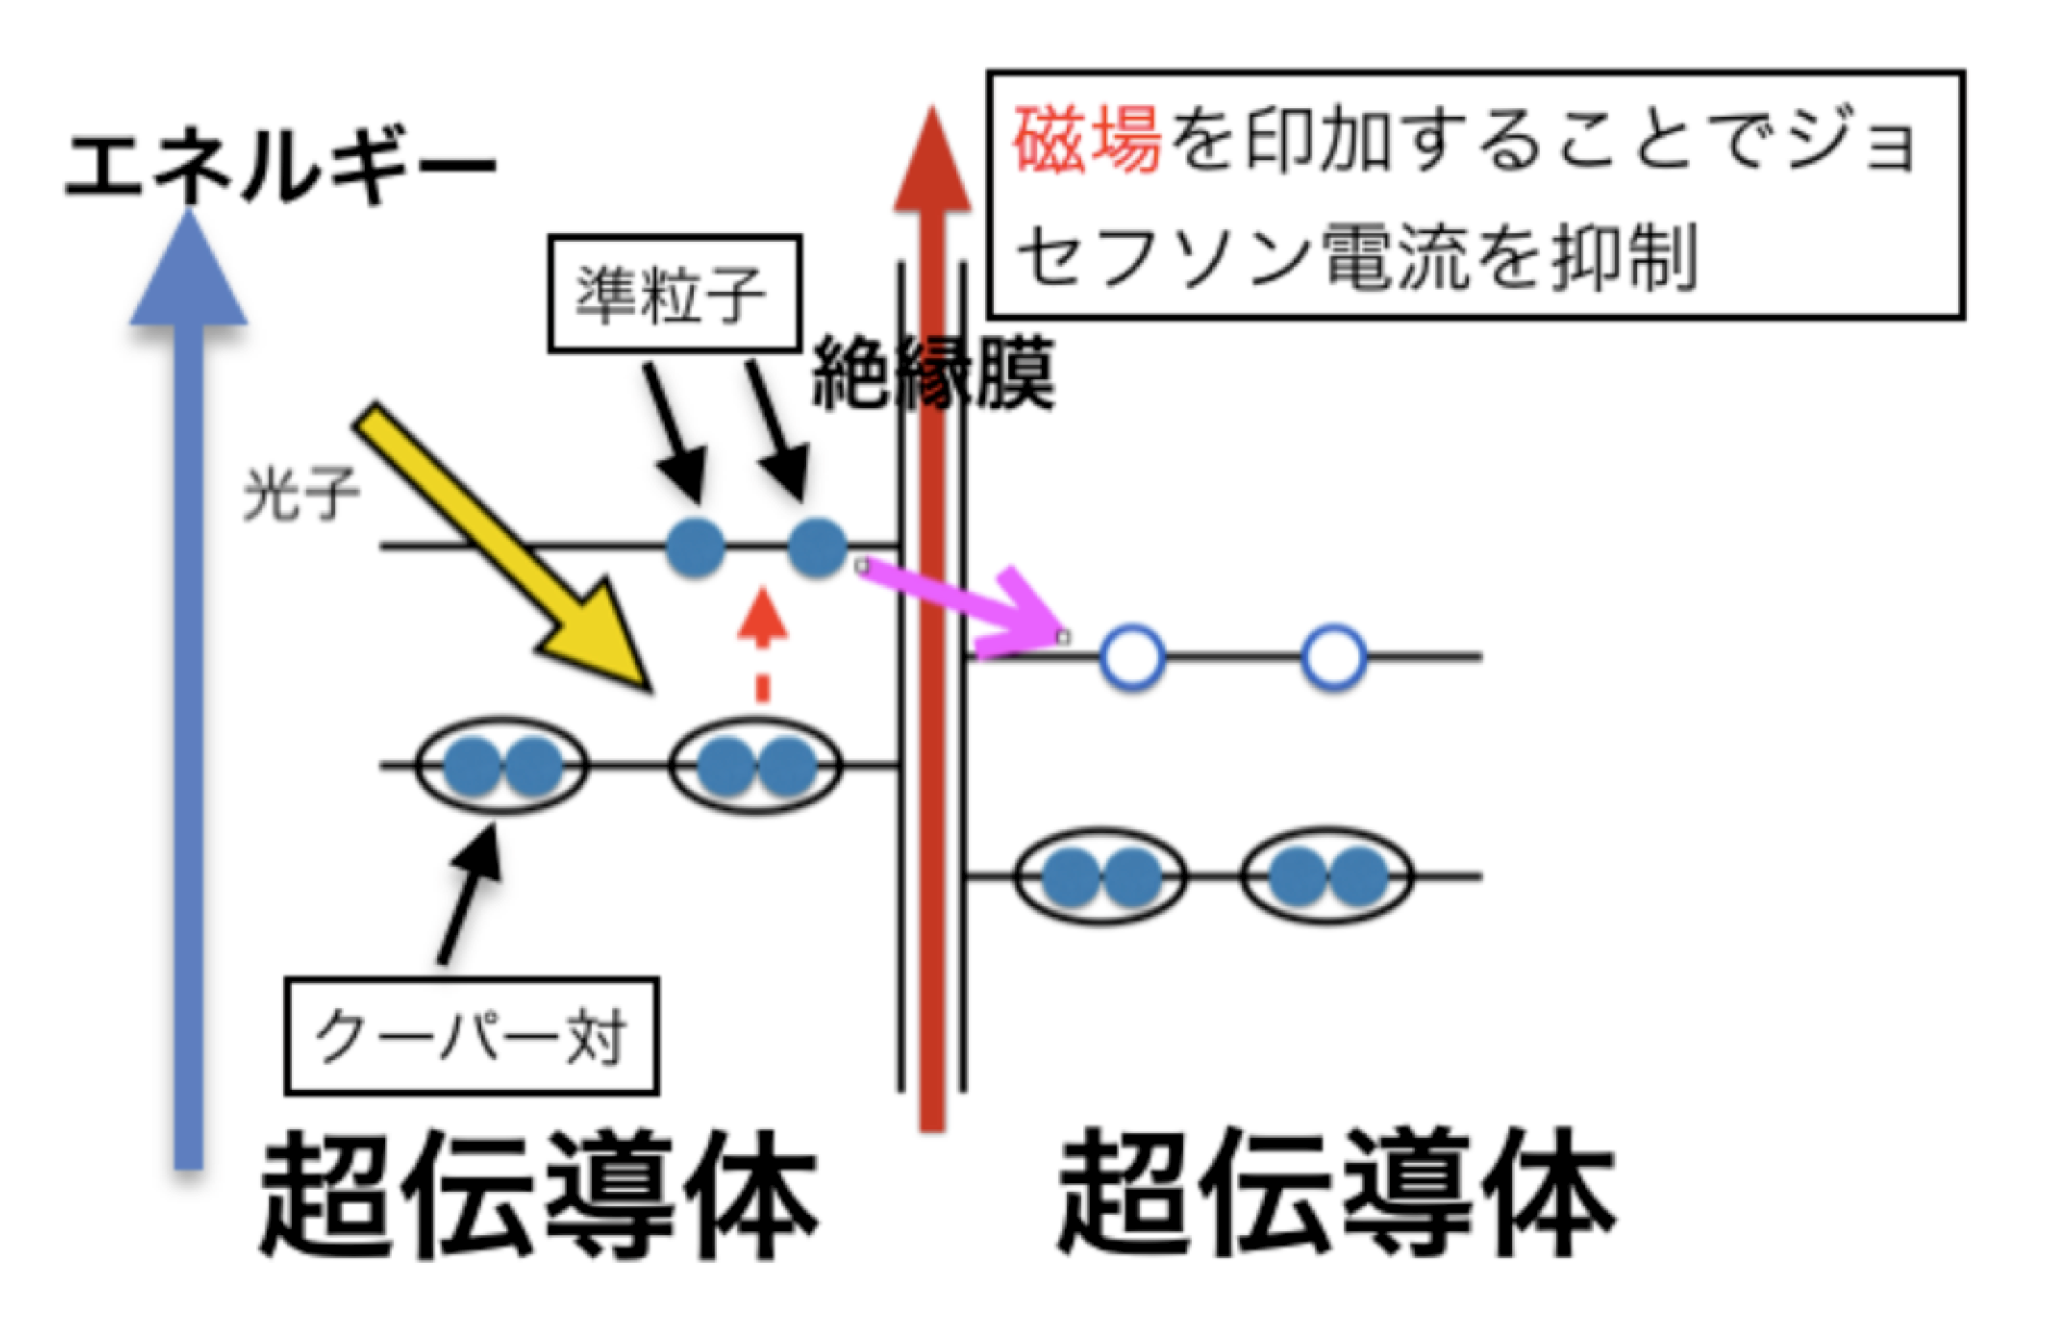
\includegraphics[width=12.0cm]{./Chapter/Chapter2/Picture/STJ_WorkingPrinciple.eps}
    				\caption{超伝導トンネル接合素子光検出器(STJ)動作原理の概念図}
    				\label{fig:STJ_WorkingPrinciple}
  			\end{center}
		\end{figure}
		STJ検出器の動作原理の概念図を図\ref{fig:STJ_WorkingPrinciple}に示す。粒子が検出器中に入射すると、超伝導体中のクーパー対が破壊され準粒子が生成される。生成された準粒子は超伝導体中を拡散し、絶縁膜に到達した準粒子はトンネル効果によって反対側の超伝導体へ通り抜ける。この準粒子のトンネル電流を信号として観測する。STJを動作する際には2つの超伝導体にバイアス電圧を印加し、2つの超伝導体の電位に勾配をつけることで絶縁膜をトンネルした準粒子の逆流を防ぐ。
		
		また、STJ検出器はSIS構造を持つので、信号とは別にジョセフソン電流も生じる。これは信号に対してバックグラウンドになるので抑制する必要がある。このジョセフソン電流は素子の絶縁膜に対して平行に磁場を印加した場合に抑制することができる。ジョセフソン電流$I_C$は磁場が存在すると、フラウンフォーファーと同型の依存性を示す。
		\begin{eqnarray}
			I_{C} = I_{C0} \left| \frac{\sin (\pi \phi / \phi_0)}{\pi \phi / \phi_0} \right|
		\end{eqnarray}
		$\phi$は印加磁場、$\phi_0$は定数である。磁場を印加することでジョセフソン電流が抑制されるので、STJ動作の際には十分な磁場を印加して、微弱な信号を観測する。
	
	\subsection{STJ検出器のエネルギー分解能}
		超伝導体状態ではフェルミオンである電子2つがフォノンを介してクーパー対を形成してボーズ粒子として振る舞う。STJを検出器として動作させる場合、入射粒子が超伝導体中のクーパー対を解離させ、2個の準粒子を生成し、それらの電子がトンネル効果で絶縁膜を通過することが必要になる。STJ信号を得るために必要な最低エネルギーは$2\Delta$である。したがって、$\Delta$が小さければ、それだけエネルギー分解能に優れた検出器ができる。STJのエネルギー分解能は式(\ref{eq:STJ_EnergyResolution})のように表される。
		\begin{eqnarray}
			\sigma_{FWHM} = \frac{\Delta N_q}{N_q} = 2.35 \sqrt{(1.7 \delta) FE}
			\label{eq:STJ_EnergyResolution}
		\end{eqnarray}
		ただし、
		\[
		\begin{cases}
			F : \mathrm{Fano\ Factor} \\
			E : \mathrm{入射粒子のエネルギー}
		\end{cases}
		\]
		である。Nb/Al-STJ検出器の場合、Fano\ Factorは0.1〜0.2程度である。式(\ref{eq:E_Tc})の関係式と照らし合わせて考察する。
		
		STJ検出器開発において、より高いエネルギー分解能が要求されるのに対し、エネルギー分解能を上げるためにエネルギーギャップが小さい超伝導体を用いようとすると、式(\ref{eq:E_Tc})から分かるように転移温度が低くなるので、より低温の測定系構築が要求されることになる。
		
	\subsection{STJのリーク電流}
		磁場を印加している場合、理想的なSTJ検出器ならば接合間に電流が流れることない。しかし、実際には以下で述べるような要因によるリーク電流が存在してしまい、これがSTJ信号のバックグラウンドとなる。
		\subsubsection{不完全な構造的な欠陥}
			酸化膜に開いた微小なピンホールや素子側面での2枚の超伝導体の接触などによるリーク電流をさす。図\ref{fig:STJ_leak_structure}にSTJ検出器の不完全な構造から生じるリーク電流の概念図を載せた。
			\begin{figure}[htbp]
  				\begin{center}
    					\includegraphics[width=12.0cm]{./Chapter/Chapter2/Picture/STJ_leak_structure.eps}
    					\caption{STJ検出器の不完全な構造起因の概念図}
    					\label{fig:STJ_leak_structure}
  				\end{center}
			\end{figure}	
		
		\subsubsection{熱励起によって生じる準粒子}
		構造的な欠陥をいくら改善しても、有限温度であれば必ず熱励起によって生じる準粒子は存在する。その準粒子がトンネル効果によって絶縁膜を流れるのならば、それはリーク電流となり得る。このリーク電流の温度依存性は理論的に計算されており、リーク電流$I_{\mathrm{leak}}$と温度$T$との関係は式(\ref{eq:STJ_leak_temp})のように書ける。\cite{13}
		\begin{eqnarray}
			I_{\mathrm{leak}} \propto T^{1/2} \exp \left(- \frac{\Delta}{k_{B}T} \right)
			\label{eq:STJ_leak_temp}
		\end{eqnarray}
		この式から、熱起因によるリーク電流は温度が下がるにつれて指数関数的に減少する。つまり、ここから言えることはSTJ検出器で十分なパフォーマンスを発揮するためには構造的な欠陥を極力抑えることに加えて、十分に冷却する必要もある。
		
		\subsubsection{その他}	
	
	\subsection{STJ検出器の電流電圧特性}
		\begin{figure}[htbp]
  			\begin{center}
    				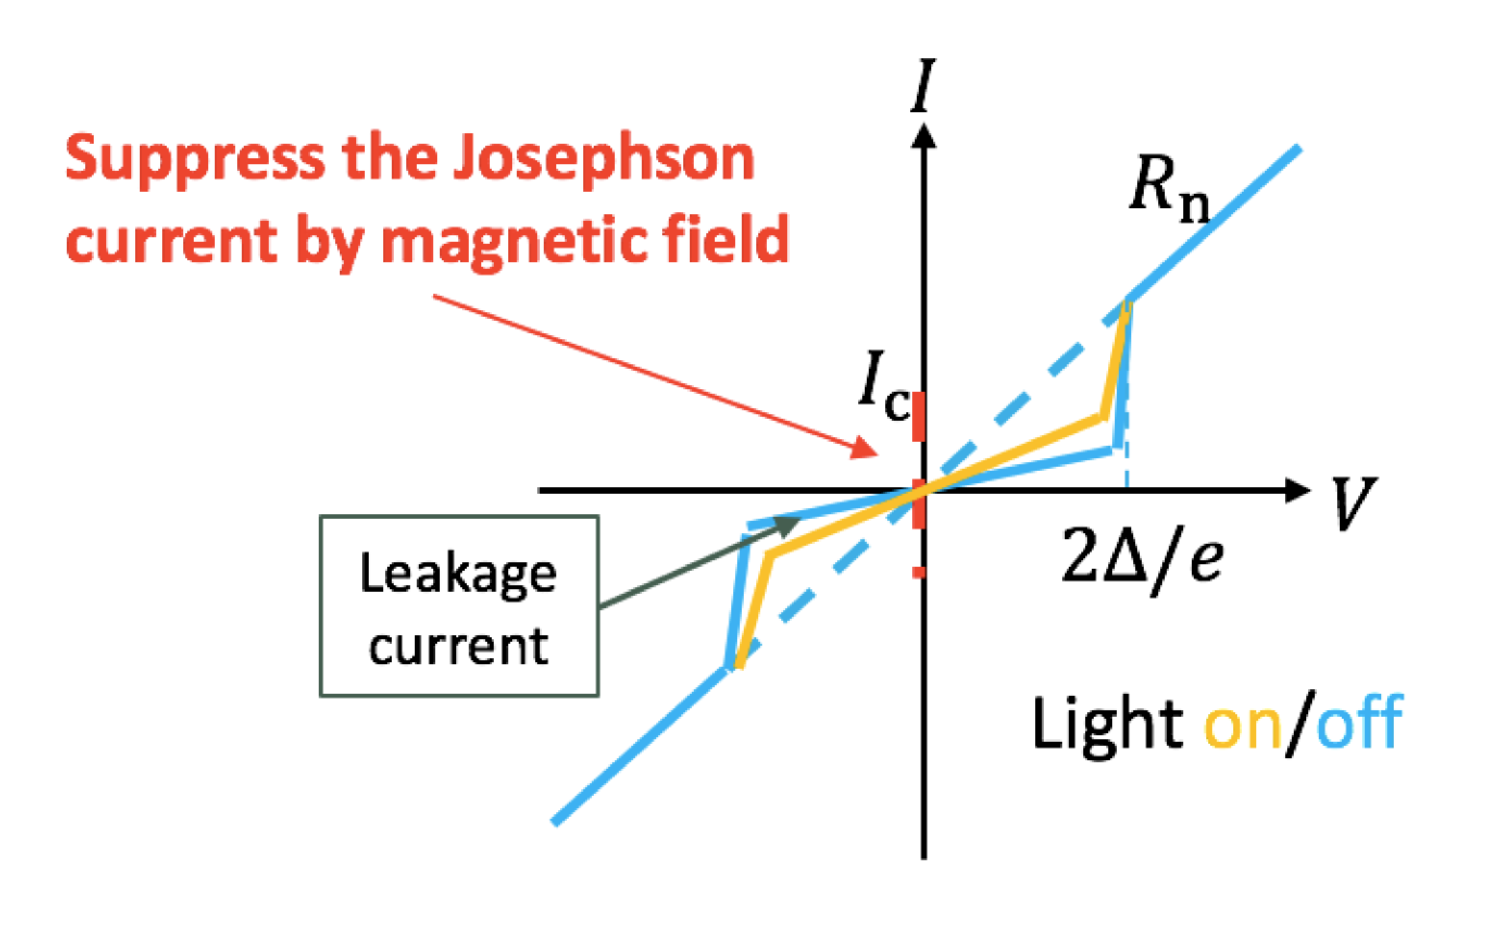
\includegraphics[width=12.0cm]{./Chapter/Chapter2/Picture/STJ_IV.eps}
    				\caption{一般的なSTJ検出器の電流電圧特性}
	  			\label{fig:STJ_IV}
  			\end{center}
		\end{figure}
		STJ検出器の電流電圧特性を図\ref{fig:STJ_IV}に示す。このSTJ検出器の電流電圧特性を測定し、素子の性能評価を行う。
		\begin{description}
			\item[$0 < |V| < 2 \Delta / e$の場合]\mbox{}\\
				クーパー対は準粒子として絶縁膜をトンネルすることができず、理想的には電流は流れない。しかし、前述したように不完全な構造や熱などに起因するリーク電流が存在するために、実際は電流はゼロにならず、有限の抵抗を持つ。この領域のことは「ダイナミックレジスタンス領域」と呼ばれ、そしてこの領域での抵抗値は$R_d$と表される。
			\item[$|V| > 2 \Delta /e$の場合]\mbox{}\\
				クーパー対はもう一方の超伝導体へトンネルすることができる。したがって、この領域での電流電圧特性は通常の抵抗のように振る舞う。この領域のことは「ノーマルレジスタンス領域」と呼ばれ、そしてこの領域での抵抗値は$R_n$と表される。
		\end{description}
		
		したがって、通常のSTJ検出器として動作させる場合は、印加電圧Vが「ダイナミックレジスタンス領域」に収まるように設定する。またSTJ検出器に光が入射した場合、クーパー対解離によって生じるトンネル電流が増加するので、図\ref{fig:STJ_IV}のように、青線から黄線に変化する。
	
\section{Nb/Al-STJ検出器}
	我々はニュートリノ崩壊光探索実験に用いるSTJ検出器として、超伝導体にハフニウムHfを用いた「Hf-STJ」と、超伝導体にニオブNbとアルミニウムAlを組み合わせた「Nb/Al-STJ」の研究開発を行っている。
	Hf-STJは、用いる超伝導体ハフニウムHfのエネルギーギャップ$\Delta$が0.020meVと非常に小さいのでエネルギー分解能に非常に優れている。我々は2012年に世界初のハフニウムHfを用いたHf-STJ検出器の作製に成功し、光に対する応答を確認した。このHf-STJは品質の良い素子作製プロセスを確立するために現在研究開発の最中である。また、これは将来の衛星実験の際に用いることを考えている。
	本節では、Hf-STJではなく、衛星実験の前実験であるロケット実験に用いるNb/Al-STJについて述べる。
	\subsection{Nb/Al-STJ検出器の構造}
		\begin{figure}[htbp]
  			\begin{center}
    				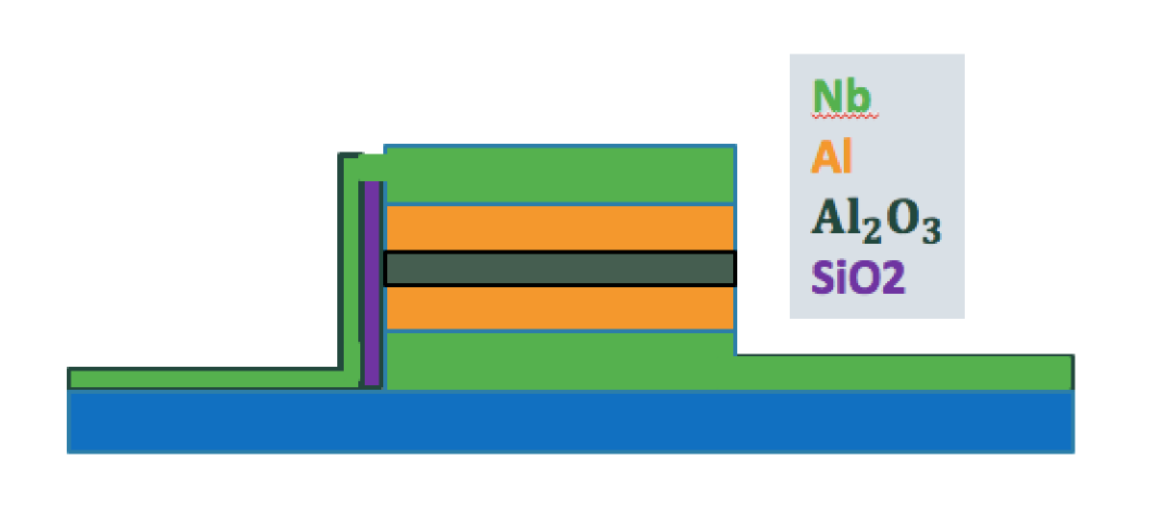
\includegraphics[width=12.0cm]{./Chapter/Chapter2/Picture/NbAlSTJ_structure.eps}
    				\caption{Nb/Al-STJ検出器の構造概念図}
	  			\label{fig:NbAlSTJ_structure}
  			\end{center}
		\end{figure}
		前述したように、Nb/Al-STJ検出器はニュートリノ崩壊光探索ロケット実験に用いる予定で、現在研究開発中である。用いる超伝導体に、ニオブNbとアルミニウムAlの2種類の超伝導体を組み合わせており、絶縁膜に酸化アルミニウム$\mathrm{Al_{2}O_3}$を用いている。Nb/Al-STJ検出器の構造を図\ref{fig:NbAlSTJ_structure}に示す。
		ニオブNb層と絶縁膜の間に、ニオブNbのエネルギーギャップ$\Delta_{\mathrm{Nb}}$に比べて更にエネルギーギャップが小さいアルミニウムAl層を挟むことによって、STJ検出器として動作させる際に有利に働く以下の特徴が現れる。
		\begin{description}
			\item[より高品質な絶縁膜の形成]\mbox{}\\
				Nb酸化膜を絶縁膜としたSTJ検出器は熱サイクルに弱く、繰り返し冷却して使用できない。一方、Al酸化膜は熱サイクルに強い。\\
				使い勝手のよいSTJ検出器を作製するために、Al酸化膜をNb系STJ検出器に用いる場合、必然的にニオブNb層とAl酸化膜の間にAl層を形成することになる。
			\item[近接効果による転移温度$T_C$とエネルギーギャップ$\Delta$の調節]\mbox{}\\
				ニオブの転移温度$T_{C\mathrm{Nb}}$が9.2Kであるのに対し、アルミニウムの転移温度$T_{C\mathrm{Al}}$は1.1Kと低い。
				2つの超伝導体を接合した場合、一方の超伝導体のクーパー対の波動関数がもう一方の超伝導体内に染み出し、転移温度が変化する。
				この効果を「近接効果」という。変化の度合いは2つの超伝導体の厚みの比率に応じて変化する。
				式(\ref{eq:E_Tc})と照らし合わせて考えると、Al層の厚さを調節することによって、転移温度と、同時にエネルギーギャップ$\Delta$を調節することができる。
				したがって、Al層を挟むことによって、Nb単体で作製されたSTJ検出器に比べてエネルギーギャップ$\Delta$は下がる。
				結果エネルギー分解能を向上させることが可能である。
			\item[バックトンネリングによるトンネル準粒子数の増加]\mbox{}\\
				\begin{figure}[htbp]
  					\begin{center}
    						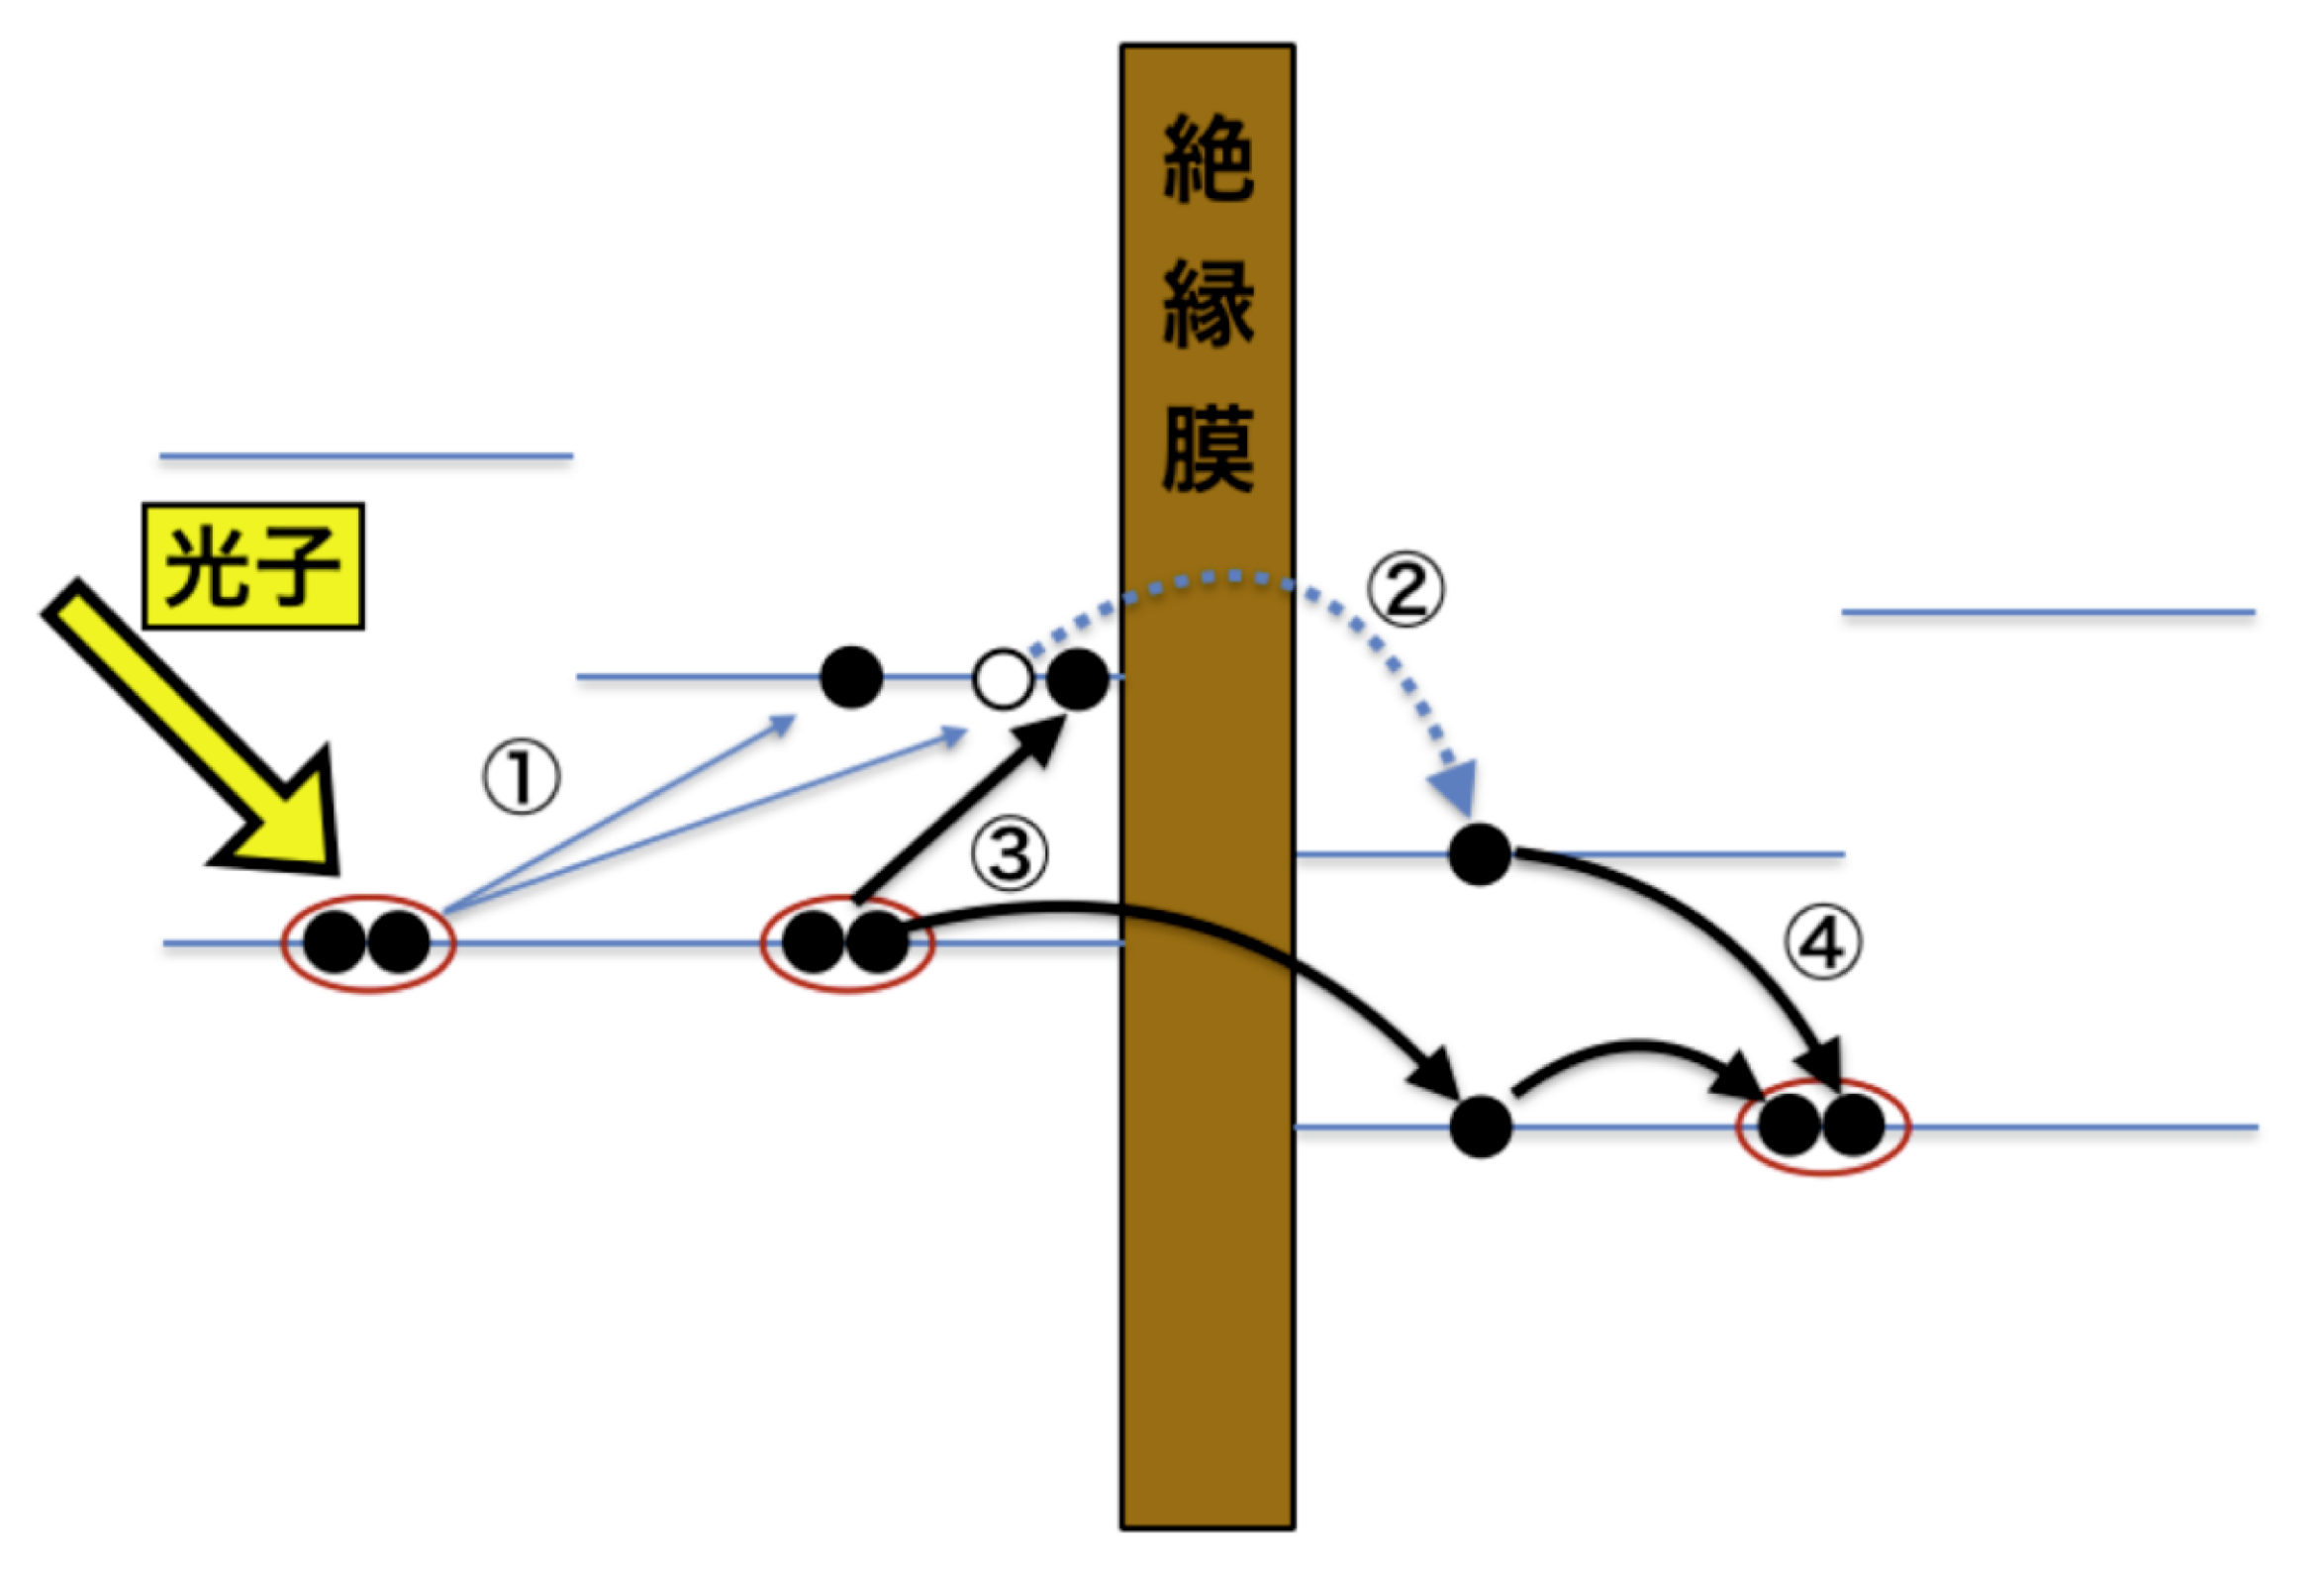
\includegraphics[width=12.0cm]{./Chapter/Chapter2/Picture/NbAlSTJ_backtunnel.eps}
    						\caption{バックトンネリング効果の概念図}
	  					\label{fig:NbAlSTJ_backtunnel}
  					\end{center}
				\end{figure}
				Nb/Al-STJ検出器のように、超伝導体と絶縁膜の間によりエネルギーギャップが小さい超伝導体を挟むことでトンネルする準粒子数が増加する、バックトンネリング効果が現れる。図\ref{fig:NbAlSTJ_backtunnel}にバックトンネリング効果の概念図を載せる。
				
				バックトンネリング効果の流れは以下のようになる。
				\begin{enumerate}
					\item STJ検出器の上部伝導体に入射した粒子がクーパー対を壊し、2つの準粒子を発生させる。
					\item 2つの準粒子のうち、1つは上部超伝導体のAl層の常伝導体にトラップされて、もう1つは絶縁膜をトンネルして下部聴伝導体のAl層の常伝導体にトラップされる。
					\item 下部超伝導体にクーパー対を作ろうと、上部伝導体の別のクーパー対が壊されて新たに2つの準粒子が生成される。
					\item 先に絶縁膜をトンネルした粒子どうしが再結合してクーパー対をなす。
					\item 残された準粒子は上部超伝導体のAl層常伝導体でトラップされる
				\end{enumerate}
				この一連の流れを繰り返すことでトンネル準粒子数が増加、つまりトンネル電流が増加する。
				バックトンネリング効果を踏まえ、STJ検出器にエネルギーEを持つ粒子が入射したときの準粒子生成個数$N$は、
				\begin{eqnarray}
					N = G_{\mathrm{Al}} \frac{E}{1.7 \Delta}
				\end{eqnarray}
				となる。この$G_{\mathrm{Al}}$をトラッピングゲインと呼び、バックトンネリング効果によるトンネル準粒子数の増加率を表す。トラッピングゲイン$G_{\mathrm{Al}}$は約10倍程度とされている。
		\end{description}

	\subsection{Nb/Al-STJ検出器の研究開発の現状}
		本研究グループは2014年度から、産業技術総合研究所(AIST)との共同研究を開始した。
		そして、Nb/Al-STJ検出器素子作製は産業技術総合研究所のCRAVITY(Clean Room for Analog-digital superconductiVITY)で行なわれている。
		ここでは安定して高品質の超伝導素子を作製することができる。
		
		図\ref{fig:NbAlSTJ_leaktemp}にCRAVITYで作製されたNb/Al-STJ検出器のリーク電流の温度依存性を示す。
		素子のサイズは$50 \times 50 \mathrm{{\mu m}^2}$である。
		この図からわかるように、0.4K程度以下でリーク電流が飽和することがわかる。この飽和したリーク電流は熱起因ではないリーク電流であり、より高品質のSTJ検出器素子作製や測定系の改善を行うことで下げることができる。
		25meVの一光子をリーク電流の揺らぎに対して$3 \sigma$以上で検出するためには、STJ検出器の信号幅を$1 \mathrm{\mu s}$と仮定すると、STJ検出器のリーク電流要求値は100pA以下である必要がある。
		表\ref{tab:NbAlSTJ_leaksize}に、我々が測定したNb/Al-STJ検出器のサイズごとのリーク電流値を示す。この表からCRAVITY製のNb/Al-STJ検出器はCOBAND実験のリーク電流の要求値を満たしていることがわかる。
		
		しかし、現在もなおNb/Al-STJ検出器を用いて遠赤外光一光子検出の成功には至っていない。その理由として、STJ検出器からの信号を冷凍機外部へと長い配線を経て読み出す際に、測定系由来の雑音がSTJ検出器信号に大きく効いてきてしまうからだ。この問題の解決策として、STJ検出器が動作する極低温環境下においても動作可能な前置増幅器を冷凍機内に設置し、STJ検出器信号が雑音に埋もれてしまう前に増幅する方法がある。\\
		我々は現在、この極低温前置増幅器の研究開発を行なっており、次章はこれについて詳しく述べる。
		%=====Nb/Al-STJのリーク電流温度依存性のplotを載せる=====%
		\begin{figure}[htbp]
  			\begin{center}
  				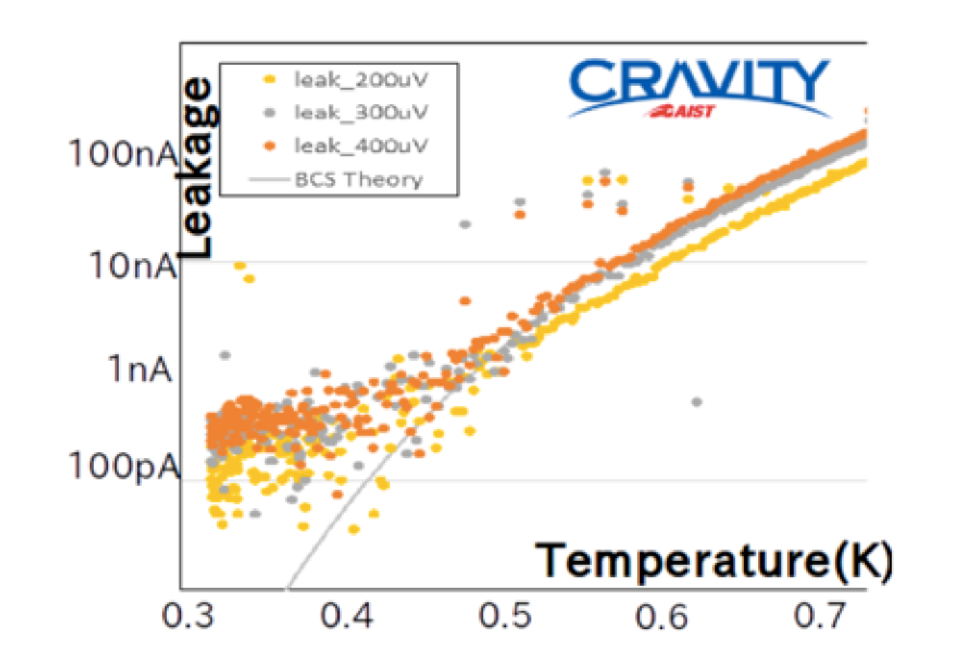
\includegraphics[width=8.0cm]{./Chapter/Chapter2/Picture/NbAlSTJ_leaktemp.eps}
    				\caption{CRAVITY製Nb/Al-STJ検出器のリーク電流温度依存性}
	  			\label{fig:NbAlSTJ_leaktemp}
 			\end{center}
		\end{figure}
		%=====現在のリーク電流の状況を表にして載せる=====%
		\begin{table}[htb]
			\begin{center}
				\caption{CRAVITY製Nb/Al-STJ検出器のサイズごとのリーク電流値}
				\begin{tabular}{| l || c | c | c |} \hline
					Nb/Al-STJのサイズ & ${100 \mathrm{\mu m}}^2$ & ${50 \mathrm{\mu m}}^2$ & ${20 \mathrm{\mu m}}^2$ \\ \hline
					リーク電流$I_{\mathrm{leak}}$@0.4mV & 2 nA & 300 pA & 100 pA \\ \hline
				\end{tabular}
				\label{tab:NbAlSTJ_leaksize}
			\end{center}
		\end{table}
	